\documentclass[english,aspectratio=169,dvipsnames]{beamer}

\usetheme[]{IKRv3}

\usepackage{etoolbox}
\usepackage{parskip}
\usepackage{marvosym}
\usepackage{changepage}
\usepackage{enumitem}
\usepackage{xcolor}
\usepackage{pgfplots}
\usepackage{xcolor}
\usepackage{amsmath}
\usepackage{pgf-pie}
\usepackage{appendixnumberbeamer}


\usetikzlibrary{positioning}
\usetikzlibrary{calc}
\usetikzlibrary{arrows}
\usetikzlibrary{arrows.meta}
\usetikzlibrary{shapes.geometric}
\usetikzlibrary{fit}
\usetikzlibrary{intersections}
\usetikzlibrary{decorations}
\usetikzlibrary{shadows.blur}
\usetikzlibrary{patterns}
\usetikzlibrary{overlay-beamer-styles}
\usetikzlibrary{matrix}


\selectcolormodel{rgb}

%catpuccin macchiatto colors
\definecolor{rosewatermacchiato}{HTML}{f4dbd6}
\definecolor{flamingomacchiato}{HTML}{f0c6c6}
\definecolor{pinkmacchiato}{HTML}{f5bde6}
\definecolor{mauvemacchiato}{HTML}{c6a0f6}
\definecolor{redmacchiato}{HTML}{ed8796}
\definecolor{maroonmacchiato}{HTML}{ee99a0}
\definecolor{peachmacchiato}{HTML}{f5a97f}
\definecolor{yellowmacchiato}{HTML}{eed49f}
\definecolor{greenmacchiato}{HTML}{a6da95}
\definecolor{tealmacchiato}{HTML}{8bd5ca}
\definecolor{skymacchiato}{HTML}{91d7e3}
\definecolor{sapphiremacchiato}{HTML}{7dc4e4}
\definecolor{bluemacchiato}{HTML}{8aadf4}
\definecolor{lavendermacchiato}{HTML}{b7bdf8}

% \definecolor{text}{HTML}{cad3f5}
% \definecolor{subtext1}{HTML}{b8c0e0}
% \definecolor{subtext0}{HTML}{a5adcb}
% \definecolor{overlay2}{HTML}{939ab7}
% \definecolor{overlay1}{HTML}{8087a2}
% \definecolor{overlay0}{HTML}{6e738d}
% \definecolor{surface2}{HTML}{5b6078}
% \definecolor{surface1}{HTML}{494d64}
% \definecolor{surface0}{HTML}{363a4f}
% \definecolor{base}{HTML}{24273a}
% \definecolor{mantle}{HTML}{1e2030}
% \definecolor{crust}{HTML}{181926}

%catpuccin latte colors
\definecolor{rosewaterlatte}{HTML}{dc8a78}
\definecolor{flamingolattele}{HTML}{dd7878}
\definecolor{pinklatte}{HTML}{ea76cb}
\definecolor{mauvelatte}{HTML}{8839ef}
\definecolor{redlatte}{HTML}{d20f39}
\definecolor{maroonlatte}{HTML}{e64553}
\definecolor{peachlatte}{HTML}{fe640b}
\definecolor{yellowlatte}{HTML}{df8e1d}
\definecolor{greenlatte}{HTML}{40a02b}
\definecolor{teallatte}{HTML}{179299}
\definecolor{sapphirelatte}{HTML}{209fb5}
\definecolor{bluelatte}{HTML}{1e66f5}
\definecolor{skylatte}{HTML}{04a5e5}
\definecolor{lavenderlatte}{HTML}{7287fd}


% policies colors
\newcommand{\kspff}{RoyalBlue}
\newcommand{\ffksp}{SkyBlue}
\newcommand{\ksplf}{YellowGreen}
\newcommand{\kspbff}{Fuchsia}
\newcommand{\kspbfl}{Thistle}
\newcommand{\kspwff}{BurntOrange}
\newcommand{\kspwfl}{Peach}


\setbeamercolor*{block title example}{fg=black,
bg=greenmacchiato}
\setbeamercolor*{block body example}{fg= black,
bg= IKRBlue!15}



\title{Designing Autoencoder Neural Networks \\ for Efficient IP-Optical Networking}
\subtitle{Master's Thesis}
\date{August 26, 2025} % defaults to \today
\author{Hakan Deli}

% \setbeamertemplate{section in toc} {
%     \hspace{0.5cm}%
%     \tikz[baseline]{
%         %\node[rectangle, fill=white, minimum width = 1mm, minimum height = 1mm] (r1) at (0,0.5) {};%
%         \node[circle, fill = IKRBlue, inner sep = 0.2mm, anchor = center] (n1) at (0,0.11) {\textcolor{white}{\inserttocsectionnumber}};}%
%         \hspace{2mm} \inserttocsection
% }

% \setbeamertemplate{subsection in toc}{\hspace{1.5cm}\inserttocsubsection\\}

\makeatletter
\patchcmd{\beamer@sectionintoc}
  {\vfill}
  {\vskip\itemsep}
  {}
  {}
\makeatother

\makeatletter
\patchcmd{\beamer@subsectionintoc}
  {\vfill}
  {\vspace{-10cm}}
  {}
  {}
\makeatother


% \setbeamertemplate{section in toc} {
%     \hspace{0.5cm} % Adjust this for consistent indentation across all levels
%     \tikz[baseline]{
%         \node[circle, fill = IKRBlue, inner sep = 0.2mm, anchor = center] (n1) at (0,0.11) {\textcolor{white}{\inserttocsectionnumber}};
%     }%
%     \hspace{2mm} \inserttocsection
% }

\setbeamertemplate{section in toc} {
    \hspace{0.5cm}\inserttocsection
}

\setbeamertemplate{subsection in toc} {
    \tab\inserttocsubsection\newline%
}

\setlist[itemize]{label=\textcolor{IKRBlue}{\textbullet}}

% \setcounter{tocdepth}{2}

\begin{document}

%bgrect tikzstyle
\tikzstyle{bgrect} = [  rectangle, 
                        fill = IKRBlue!20, 
                        minimum width = 14cm, 
                        minimum height = 6.9cm, 
                        rounded corners = 5pt, %5pt
                        anchor = north west]
\tikzstyle{bgrectw} = [ rectangle, 
                        fill = white, 
                        minimum width = 14cm, 
                        minimum height = 6.9cm, 
                        rounded corners = 5pt, %5pt 
                        anchor = north west]

\begin{frame}[plain]{Outline}
    \vspace{0.3cm}
    \begin{minipage}[t][1cm][t]{\linewidth}
        \setlength{\itemsep}{0cm}
        \setlength{\parskip}{3pt} 
        \tableofcontents[sectionstyle=show,subsectionstyle=show,subsubsectionstyle=hide]
    \end{minipage}
\end{frame}

\breadcrumbson

\section{Motivation}

\begin{frame}{Motivation}
    \vspace{0cm}
    % \only<2->{
    % \begin{textblock}{5}(0.4, 1.36)
    %     \begin{tikzpicture}
    %         \node[bgrect, minimum width = 7.6cm, minimum height = 6.3cm, anchor = center] at (0, 0) {};
    %     \end{tikzpicture}
    % \end{textblock}
    % }
    \only<2->{
    \begin{textblock}{5}(0.6, 1.5)
        \begin{tikzpicture}
            \node[bgrectw, minimum width = 7.2cm, minimum height = 6.5mm, anchor = center] at (0, 0) {};
        \end{tikzpicture}
    \end{textblock}
    }
    \only<3->{
    \begin{textblock}{5}(0.6, 2.28)
        \begin{tikzpicture}
            \node[bgrectw, minimum width = 7.2cm, minimum height = 2.2cm, anchor = center] at (0, 0) {};
        \end{tikzpicture}
    \end{textblock}
    }
    \only<4->{
    \begin{textblock}{5}(0.6, 4.6)
        \begin{tikzpicture}
            \node[bgrectw, minimum width = 7.2cm, minimum height = 2.9cm, anchor = center] at (0, 0) {};
        \end{tikzpicture}
    \end{textblock}
    }
    \begin{columns}
        \column{0.5\textwidth}
            \vspace{0.3cm}
            \begin{textblock}{6.5}(1.0, 1.55)
                \begin{itemize}
                    \setlength\itemsep{1em}
                    \visible<2->{\item[]\hspace{-7mm} \textbf{Growing Volume of Internet Traffic Worldwide}}
                    \visible<3->{\item[]\hspace{-7mm} \textbf{Optical Networks}}
                    \visible<3->{\item for long distances (countries, continents...)}
                    \visible<3->{\item indispensable for everydays communication}
                    \visible<4->{\item[]\hspace{-7mm} \textbf{Network Operators Need to Route Traffic}}
                    \visible<4->{\item decision highly impacts performance}
                    \visible<4->{\item affects energy consumption, data rate, ...}
                    \visible<4->{\item heuristic methods usually used}
                \end{itemize}
            \end{textblock}
        \column{0.5\textwidth}
        \only<2-> {
            \vspace{0cm}
            \begin{figure}[ht]
    	       \begin{adjustwidth}{0cm}{0cm}
        		\centering
        		

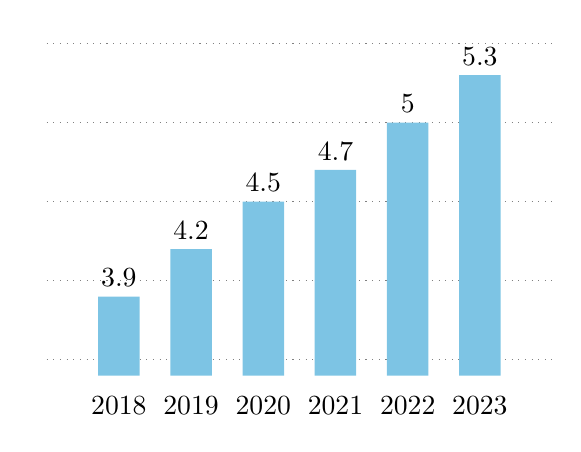
\begin{tikzpicture}
  \begin{axis}[
    ybar,
    bar width=12pt,
    ymin=3.4,
    ymax=5.6,
    ylabel={},
    xlabel={},
    xtick=data, 
    ymajorgrids,
    grid style={dotted,gray},
    y axis line style = {draw = none},
    tick style = {draw=none},
    xticklabel pos = bottom,
    xtick pos = bottom,
    ytick pos = left,
    yticklabels=\empty,
    bar width = 15pt,
    xticklabels={2018,2019,2020,2021,2022,2023},
    nodes near coords,
    nodes near coords align={vertical},
    enlarge x limits=0.2,
    width=8cm, height=6cm
  ]

    \addplot[fill=sapphiremacchiato, draw=none] coordinates {
      (2018,3.9)
      (2019,4.2)
      (2020,4.5)
      (2021,4.7)
      (2022,5.0)
      (2023,5.3)
    };
  \end{axis}
\end{tikzpicture}


        		\vspace{0cm}
                \captionsetup{justification=centering}
        		\caption*{
                        % \begin{center} 
                        number of Internet users from 2018 - 2023 \\ (adopted from the Cisco annual Internet report) 
                        % \end{center}
                        }
    	       \end{adjustwidth}
            \end{figure}
        }
    \end{columns}
\end{frame}


\begin{frame}{Deep Learning (DL)}
    
    \begin{textblock}{5}(0.36, 1.4)
        \begin{tikzpicture}[x=5cm, 
                    y=1.5cm, 
                    arrow/.style={->, draw = black, line width = 0.5pt, > = Stealth},
                    arrowbold/.style={-{Triangle[length=3mm, width=5mm]}, draw = MidnightBlue!60, line width = 5pt},
                    on grid]
    \node[bgrect, minimum width = 15.21cm, minimum height = 5cm, anchor = center] at (0, 0) {};

    \node[bgrectw, minimum width = 14.5cm, minimum height = 0.7cm, align = center, anchor = center, visible on = <1->] (n1) at (0, 1) {advances in machine learning $\rightarrow$ new possibilities};
    \node[bgrectw, minimum width = 4.4cm, minimum height = 1.2cm, align = center, anchor = center, visible on = <2->] (n2) at (-1, -0.7) {reinforcement \\ learning};
    \node[bgrectw, minimum width = 3.5cm, minimum height = 1.2cm, align = center, anchor = center, visible on = <2->] (n3) at (0, -0.7) {How to incorporate \\ the potential optimum?};
    \node[bgrectw, minimum width = 4.4cm, minimum height = 1.2cm, align = center, anchor = center, visible on = <3->] (n4) at (1, -0.7) {supervised DL};
    % \node[bgrectw, minimum width = 8.7cm, minimum height = 1.2cm, align = center, anchor = center, visible on = <3->] (n5) at (0.57, -1.1) {deep neural networks (DNNs) learn \\ from precomputed optimum};
    % \node[bgrectw, minimum width = 4.4cm, minimum height = 1.2cm, align = center, anchor = center, visible on = <3->] (n6) at (-1, -1.1) {act in \\ real-time};

    \draw[arrowbold, shorten <= 3mm, shorten >= 3mm, visible on = <2->] (n2.north)++(0,1.05) -- node[right, xshift = 2mm] {current research} (n2.north);
    \draw[arrow,  visible on = <2->] (n2) -- (n3);
    \draw[arrow,  visible on = <3->] (n3) -- (n4);
    \draw[arrowbold, shorten <= 3mm, shorten >= 3mm, visible on = <3->] (n4.north)++(0,1.05) -- node[right, xshift = 2mm] {this thesis} (n4.north);
    % \draw[arrow,  visible on = <3->] (n4.south) -- ($(n4.south)+(0,-0.29)$);
    % \draw[arrow,  visible on = <3->] (n5) -- (n6);
    
\end{tikzpicture}

  % \begin{adjustwidth}{6mm}{2cm}
  %               \begin{itemize}
  %                   \setlength\itemsep{1em}
  %                   \visible<2->{\item usually heuristic methods used for decision}
  %                   \visible<3->{\item advances in machine learning (ML) -> new possibilities}
  %                   \visible<4->{\item current research mainly applies reinforcement learning (RL), little to no research on supervised learning with labeled datasets}
  %                   \visible<5->{\item deep learning (DL) has the potential to incorporate optimal decisions that can be precomputed but then be applied in real time by a deep neural network (DNN)}
  %               \end{itemize}
  %   \end{adjustwidth}
    \end{textblock}

    \begin{textblock}{14.96}(0.486, 6.5)
        \visible<4-> {
          \begin{exampleblock}{\centering First Thesis Goal}
            \centering derive a DL based decision finding algorithm for network routing
          \end{exampleblock}
        }
    \end{textblock}
    
    

\end{frame}


\begin{frame}{Autoencoders}

    \only<2->{
        \begin{textblock}{5}(1, 2)
            \begin{tikzpicture}
                \node[bgrect, minimum width = 4cm, minimum height = 3.3cm, anchor = center, align = center] at (0, 0) {complexity \\ reduction};
            \end{tikzpicture}
        \end{textblock}
    }

    \only<3->{
    \begin{textblock}{5}(6, 2)
        \begin{tikzpicture}
            \node[bgrect, minimum width = 4cm, minimum height = 3.3cm, anchor = center, align = center] at (0, 0) {dimension \\ unification};
        \end{tikzpicture}
    \end{textblock}
    }

    \only<4->{
    \begin{textblock}{5}(11, 2)
        \begin{tikzpicture}
            \node[bgrect, minimum width = 4cm, minimum height = 3.3cm, anchor = center, align = center] at (0, 0) {performance \\ increase};
        \end{tikzpicture}
    \end{textblock}
    }

    \only<5->{
    \begin{textblock}{13.7}(1.14, 5.5)
            \begin{exampleblock}{\centering Second Thesis Goal}
                \centering leverage autoencoders and examine their effect on performance
            \end{exampleblock}
    \end{textblock}
    }
  
\end{frame}


\section{Theoretical Background}


\subsection{Optical Networks and the RSA Problem}

\begin{frame}{Optical Network Topology}
    \vspace{0.2cm}
    \begin{figure}
    	\begin{adjustwidth}{0cm}{0cm}
    		\centering
    		\tikzstyle{netnode} = [circle, 
					   minimum width = 0.75cm, 
					   minimum height = 0.75cm, 
					   text = black!100, 
					   align=center, 
					   line width = 1, 
					   inner sep = 1mm, 
					   shading=radial, 
					   inner color = sapphiremacchiato!50, 
					   outer color = sapphiremacchiato!100]

\tikzstyle{edge}=[> = stealth, line width = 0.5pt, shorten <= 0mm, shorten >= 0mm]
\tikzstyle{arrow}=[> = stealth, line width = 0.5pt]


\begin{tikzpicture}[x=2cm, y = 2cm]
	
	%Layer42
	\node[netnode, visible on = <2->] (nA) at (-0.53, 1.29) {A};
	\node[netnode, visible on = <2->] (nB) at (-0.35, 0.21) {B};
	\node[netnode, visible on = <4->] (nC) at (-1.39, -0.16) {C};
	\node[netnode, visible on = <4->] (nD) at (0.26, -0.68) {D};
	\node[netnode, visible on = <4->] (nE) at (1.29, -0.76) {E};
	\node[netnode, visible on = <4->] (nF) at (0.72, 0.1) {F};
	
	\draw[edge, <->, visible on = <3->] (nA) -- (nB); 
	\draw[edge, <->, visible on = <4->] (nB) -- (nC);
	\draw[edge, <->, visible on = <4->] (nB) -- (nF);
	\draw[edge, <->, visible on = <4->] (nB) -- (nD);
	\draw[edge, <->, visible on = <4->] (nD) -- (nF);
	\draw[edge, <->, visible on = <4->] (nD) -- (nE);
	\draw[edge, <->, visible on = <4->] (nE) -- (nF);   
	
	\node[align = center, visible on = <2->] (ntext) at (-1.5, 1.1) {node};
	\node[align = center, visible on = <3->] (nlink) at (0.6, 0.85) {optical \\ link};
	
	
	\draw[->, arrow, shorten <= 0.5mm, shorten >= 0.5mm, dashed, red, visible on = <2->] ($ (ntext.east) + (0, 0.03)$) -- ($ (nA.west) + (0, -0.04)$);
	\draw[->, arrow, shorten <= 5mm, shorten >= 1mm, dashed, red, visible on = <3->] ($ (nlink.center) + (0, 0)$) -- (-0.4, 0.7); 
	
	\node[align=center, baseline, visible on = <4->] (t1) at (0, -1.3) {\textbf{Layer42}};
	
	%Mren
	\node[netnode, visible on = <5->] (nAM) at (3.5, 0.29 + 1) {A};
	\node[netnode, visible on = <5->] (nBM) at (4, 0.3) {B};
	\node[netnode, visible on = <5->] (nCM) at (4-1, -0.2) {C};
	\node[netnode, visible on = <5->] (nDM) at (4+1, 0.8) {D};
	\node[netnode, visible on = <5->] (nEM) at (4.5, 0.3 - 1) {E};
	
	\draw[edge, <->, visible on = <5->] (nAM) -- (nBM); 
	\draw[edge, <->, visible on = <5->] (nBM) -- (nCM);
	\draw[edge, <->, visible on = <5->] (nBM) -- (nDM);
	\draw[edge, <->, visible on = <5->] (nBM) -- (nEM);
	
	\node[align=center, baseline, visible on = <5->] (t1) at (4, -1.3) {\textbf{Mren}};
	     
	 
\end{tikzpicture}

            \only<4->{\caption*{Network topologies from topology-zoo.org}}
    	\end{adjustwidth}
    \end{figure}
\end{frame}

\begin{frame}
    \frametitle{\large Wavelength-Division Multiplexing (WDM) and Elastic Optical Networks (EONs)}
    \begin{textblock}{5}(0.4, 1.8)
        \newcommand{\slotheight}{2cm}
\newcommand{\slotwidth}{2mm}
\newcommand{\numchannels}{10}
\newcommand{\fsperchannel}{5}
\newcommand{\lw}{1pt}

\tikzstyle{slot} = [draw = black,
					minimum width = \slotwidth, 
				    minimum height = \slotheight, 
					text = black!100, 
					anchor = west, 
					line width = \lw,
					inner sep = 0mm]
					
\tikzstyle{legendtext} = [text = black,
						  anchor = north, 
						  align = center, 
						  inner sep = 0mm,
						  font = \scriptsize]

\tikzstyle{arrow}=[> = stealth, line width = 0.5pt, dashed, red]

%{coordinate}{amount of fs}{color}{height}
\newcommand{\spectrum}[4]{%
	\path (#1) coordinate (start);
	\fill[fill opacity=0.5, fill=#3]
	($(start) + (0, \lw)$)
	-- ($ (start) + (#2*0.5*\slotwidth-0.5*\lw,\lw) $)
	arc[start angle=0, end angle=180, x radius=#2*0.5*\slotwidth-0.5*\lw, y radius=#4-\lw]
	-- cycle;
}

\newcommand{\oneslot}[2]{
	\spectrum{#1}{1}{blue}{#2}
}

\newcommand{\twoslot}[2]{
	\spectrum{#1}{2}{blue}{#2}
}

\newcommand{\threeslot}[2]{
	\spectrum{#1}{3}{violet}{#2}
}

\newcommand{\fourslot}[2]{
	\spectrum{#1}{4}{ForestGreen}{#2}
}

\newcommand{\fiveslot}[2]{
	\spectrum{#1}{5}{red}{#2}
}

\newcommand{\twelveslot}[2]{
	\spectrum{#1}{12}{orange}{#2}
}



%\tikzstyle{edge}=[> = stealth, line width = 0.5pt, shorten <= 0mm, shorten >= 0mm]
%\tikzstyle{arrow}=[> = stealth, line width = 0.5pt]

\begin{tikzpicture}[x=1cm, y=1cm]
	
	
	%WDM

    \node[draw = black, 
          minimum width = 10*\slotwidth*\fsperchannel, 
		   minimum height = \slotheight, 
		   text = black!100, 
		   anchor = west, 
		   line width = \lw,
		   inner sep = 0mm, visible on = <2>] (startbox) at (0, -0.4) {};
    
	\foreach \i in {1,...,\numchannels}{
		\pgfmathtruncatemacro{\j}{\i-1}
		\node[slot, minimum width = \slotwidth*\fsperchannel, visible on = <3->] (wdm\i) at (\j*\slotwidth*\fsperchannel, -0.4) {};
	}
	
	\node[text = black, left = 0.5cm of wdm1.west, anchor = east, visible on = <3->] (wdmtext) {WDM};
	
	%WDM spectras
	\visible<5->{\threeslot{wdm1.south}{0.98*\slotheight}}
	\visible<5->{\fiveslot{wdm2.south}{0.98*\slotheight}}
	\visible<5->{\twoslot{wdm3.south}{0.98*\slotheight}}
	\visible<5->{\fourslot{wdm7.south}{0.98*\slotheight}}
	\visible<5->{\fourslot{wdm8.south}{0.98*\slotheight}}
	\visible<5->{\twoslot{wdm9.south}{0.98*\slotheight}}
	
	%cut the top off
%	\draw[-, draw=white, line width=1mm, align=center] (wdm1.north west) -- (wdm\numchannels.north east);	
	
	%EON
    
	\pgfmathtruncatemacro{\amount}{\numchannels*\fsperchannel}
	\foreach \i in {1,...,\amount}{
		\pgfmathtruncatemacro{\j}{\i-1}
		\node[slot, minimum width = \slotwidth, draw = black!20, line width = 0.5*\lw, visible on = <7->] (fs\i) at (\j*\slotwidth+0.125*\lw, -3.4) {};
	}
	
	\node[text = black, left = 0.5cm+0.5*\lw of fs1.west, anchor = east, visible on = <7->] (eontext) {EON};
	
	%draw eon channels by hand	
	\foreach \ns/\nend in  {fs1/fs3,
						    fs4/fs8,
	                        fs9/fs10,
	                        fs11/fs22,
	                        fs23/fs30,
	                        fs31/fs34,
	                        fs35/fs38,
	                        fs39/fs40,
	                        fs41/fs50}{

	\draw[-, draw=black, line width=\lw, align=center, visible on = <9->] (\ns.north west)++(0.25*\lw,0) -- ($(\ns.south west)+(0.25*\lw, 0.5*\lw)$) -- ($(\nend.south east) + (-0.25*\lw, 0.5*\lw)$) -- ($(\nend.north east)+(-0.25*\lw,0)$);
	                        
	}

	%eon spectra
	\visible<9->{\threeslot{fs2.south}{0.98*\slotheight}}
	\visible<9->{\fiveslot{fs6.south}{0.98*\slotheight}}
	\visible<9->{\twoslot{fs9.south east}{0.98*\slotheight}}
	\visible<9->{\twelveslot{fs16.south east}{0.98*\slotheight}}
	\visible<9->{\fourslot{fs32.south east}{0.98*\slotheight}}
	\visible<9->{\fourslot{fs36.south east}{0.98*\slotheight}}
	\visible<9->{\twoslot{fs39.south east}{0.98*\slotheight}}
	
	%legend
	\foreach \y in {1,2,...,5}{
		\node[inner sep = 0mm, anchor = center, visible on = <5->] (l\y) at (12,-1.3*\y+1.8) {};
	}
	
	\node[legendtext, below = 1pt of l1.south, visible on = <5->] {25 GHz};
	\node[legendtext, below = 1pt of l2.south, visible on = <5->] {37.5 GHz};
	\node[legendtext, below = 1pt of l3.south, visible on = <5->] {50 GHz};
	\node[legendtext, below = 1pt of l4.south, visible on = <5->] {62.5 GHz};
	\node[legendtext, below = 1pt of l5.south, visible on = <5->] {150 GHz};
	
	\visible<5->{\twoslot{l1.center}{0.2*\slotheight}}
	\visible<5->{\threeslot{l2.center}{0.2*\slotheight}}
	\visible<5->{\fourslot{l3.center}{0.2*\slotheight}}
	\visible<5->{\fiveslot{l4.center}{0.2*\slotheight}}
	\visible<5->{\twelveslot{l5.center}{0.2*\slotheight}}

    \node[draw = black, 
          minimum width = 10*\slotwidth*\fsperchannel, 
		   minimum height = \slotheight, 
		   text = black!100, 
		   anchor = west, 
		   line width = \lw,
		   inner sep = 0mm, visible on = <6->] (startboxeon) at (-0.005, -3.4) {};
    
	%highlight one frequency slot and one optical channel
	\node[slot, minimum width = \slotwidth, draw = red, line width = 1.25*\lw, left = 0cm of fs44.west, anchor = west, pattern = north east lines, pattern color = red, visible on = <8->] (fsred) {};
	\node[slot, minimum width = \slotwidth*\fsperchannel, draw = red, line width = 1.25*\lw, left = 0cm of wdm5.west, anchor = west, pattern = north east lines, pattern color = red, visible on = <4->] (wdmred) {};
	
	%add arrows and explanatory text
	\node[legendtext, font = \normalsize, visible on = <4->] (wdmarrowtext) at (4.5,-1.55) {\small one WDM channel};
	\node[legendtext, font = \normalsize, align = center, visible on = <8->] (eonarrowtext) at (8.71,-4.7) {\small one FS \\ \small (12.5 GHz)};
	
	\draw[->, draw = gray, > = stealth, line width = 0.5pt, visible on = <2->] (-0.1,-1.9) -- (10.2,-1.9) node[right] {\textcolor{gray}{$\lambda$}};
    
	
	
\end{tikzpicture}
    \end{textblock}
\end{frame}

\begin{frame}{Optical Networks and the RSA Problem}
	\begin{textblock}{5}(1, 1.4)
        \tikzstyle{netnode} = [circle, 
					   minimum width = 0.25cm, 
					   minimum height = 0.25cm, 
					   text = black!100, 
					   align=center, 
					   line width = 1, 
					   inner sep = 0.5mm, 
					   shading=radial, 
					   inner color = sapphiremacchiato!50, 
					   outer color = sapphiremacchiato!100]

\tikzstyle{edge}=[> = stealth, line width = 0.3pt, shorten <= 0mm, shorten >= 0mm]


\newcommand{\slotheight}{1.2cm}
\newcommand{\slotwidth}{1mm}
\newcommand{\numchannels}{10}
\newcommand{\fsperchannel}{5}
\newcommand{\lw}{1pt}

\tikzstyle{slot} = [draw = black,
					minimum width = \slotwidth, 
				    minimum height = \slotheight, 
					text = black!100, 
					anchor = west, 
					line width = \lw,
					inner sep = 0mm]

    
\begin{tikzpicture}

    %background rectangles
    \node[rectangle, fill = IKRBlue!20, minimum width = 14cm, minimum height = 6.9cm, rounded corners = 5pt, anchor = north west, visible on = <2->] at (0,0) {};
    \node[rectangle, fill = white, minimum width = 6cm, minimum height = 3cm, rounded corners = 5pt, anchor = north west, visible on = <3->] at (0.5,-0.8) {};
    \node[rectangle, fill = white, minimum width = 6cm, minimum height = 3cm, rounded corners = 5pt, anchor = north west, visible on = <5->] at (7.5,-0.8) {};

    %plus
    \begin{scope}[shift={(7cm,-2.3cm)}, visible on = <5->]
          \def\arm{0.05}   % half-width of arms
          \def\len{0.2}     % half-length of plus arms
          % Draw filled plus shape centered at (0,0)
          \filldraw[IKRBlue]
          (-\arm, -\len) rectangle (\arm, \len)  % vertical bar
          (-\len, -\arm) rectangle (\len, \arm); % horizontal bar
    \end{scope}

    %text
    \node[anchor = west, visible on = <2->] at (0.2, -0.45) {\textbf{R}outing and \textbf{S}pectrum \textbf{A}ssignment Problem};
    \node[anchor = center, align = center, visible on = <3->] at (3.4, -4.15) {Route};
    \node[anchor = center, align = center, visible on = <5->] at (10.5, -4.15) {Spectrum};

    %layer42
    \begin{scope}[x=1.3cm, y=1.1cm, shift={(3.5cm, -2.6cm)}]
    
        %vanilla
        \node[netnode, visible on = <3->] (nA) at (-0.53, 1.29) {\small A};
        \node[netnode, visible on = <3>] (nB) at (-0.35, 0.21) {\small B};
        \node[netnode, visible on = <3->] (nC) at (-1.39, -0.16) {\small C};
        \node[netnode, visible on = <3->] (nD) at (0.26, -0.68) {\small D};
        \node[netnode, visible on = <3->] (nE) at (1.29, -0.76) {\small E};
        \node[netnode, visible on = <3>] (nF) at (0.72, 0.1) {\small F};
        
        \draw[edge, <->, visible on = <3>] (nA) -- (nB); 
        \draw[edge, <->, visible on = <3>] (nB) -- (nC);
        \draw[edge, <->, visible on = <3>] (nB) -- (nF);
        \draw[edge, <->, visible on = <3>] (nB) -- (nD);
        \draw[edge, <->, visible on = <3>] (nD) -- (nF);
        \draw[edge, <->, visible on = <3>] (nD) -- (nE);
        \draw[edge, <->, visible on = <3>] (nE) -- (nF);  
    
        %scenario
        \node[  netnode, 
                inner color = red!20, 
				outer color = red!70,
                visible on = <4->] (nBs) at (-0.35, 0.21) {\small B};

        \node[  netnode, 
                inner color = red!20, 
				outer color = red!70,
                visible on = <4->] (nFs) at (0.72, 0.1) {\small F};

        \draw[edge, <->, opacity = 0.3, visible on = <4->] (nA) -- (nB); 
        \draw[edge, <->, opacity = 0.3, visible on = <4->] (nB) -- (nC);
        \draw[edge, draw = ForestGreen, ->, visible on = <4->] (nB) -- (nF);
        \draw[edge, draw = Orchid, ->, visible on = <4->] (nB) -- (nD);
        \draw[edge, draw = Orchid, ->, visible on = <4->] (nD) -- (nF);
        \draw[edge, <->, opacity = 0.3, visible on = <4->] (nD) -- (nE);
        \draw[edge, <->, opacity = 0.3, visible on = <4->] (nE) -- (nF); 
        
    \end{scope}

    %spectrum

    \begin{scope}[shift={(8cm,-2.5cm)}]
    
        %EON
    	\pgfmathtruncatemacro{\amount}{\numchannels*\fsperchannel}
    	\foreach \i in {1,...,\amount}{
    		\pgfmathtruncatemacro{\j}{\i-1}
    		\node[slot, minimum width = \slotwidth, draw = black!20, line width = 0.5*\lw, visible on = <5->] (fs\i) at (\j*\slotwidth+0.125*\lw, 0) {};
    	}
    	
    	%draw eon channels by hand	
    	\foreach \ns/\nend in  {fs1/fs3,
    						    fs7/fs10,
    	                        fs23/fs28,
    	                        fs41/fs50}{
    
    	\fill[fill=red, opacity = 0.5, visible on = <5->] (\ns.north west)++(0.25*\lw,0) -- ($(\ns.south west)+(0.25*\lw, 0.5*\lw)$) -- ($(\nend.south east) + (-0.25*\lw, 0.5*\lw)$) -- ($(\nend.north east)+(-0.25*\lw,0)$) -- cycle;
    	                        
    	}
    
        \node[draw = black, 
              minimum width = 10*\slotwidth*\fsperchannel, 
    		   minimum height = \slotheight, 
    		   text = black!100, 
    		   anchor = west, 
    		   line width = \lw,
    		   inner sep = 0mm, visible on = <5->] (startboxeon) at (-0.005, 0) {};

        \draw[->, line width = 1pt, draw = red, > = Stealth , shorten >= 0.5mm, visible on = <6->] ($(fs13.north) + (0, 0.6)$) -- (fs13.north);
    
    \end{scope}


    % constraints
    \node[rectangle, fill = IKRBlue!5, minimum width = 4.4cm, minimum height = 2cm, rounded corners = 5pt, anchor = north west, align = center, text height = 1cm, text depth = 0.5cm, visible on = <7->] at (0.2,-4.7) {FS $\leftrightarrow$ optical channel};
    \node[rectangle, fill = IKRBlue!5, minimum width = 4.4cm, minimum height = 2cm, rounded corners = 5pt, anchor = north west, align = center, text height = 1cm, text depth = 0.5cm, visible on = <8->] at (4.8,-4.7) {no wavelength conversion};
    \node[rectangle, fill = IKRBlue!5, minimum width = 4.4cm, minimum height = 2cm, rounded corners = 5pt, anchor = north west, align = center, text height = 1cm, text depth = 0cm, visible on = <9->] at (9.4,-4.7) {assigned FSs are \\ adjacent};

    \node[anchor = center, align = center, visible on = <7->] at (2.4, -5.2) {\textbf{Capacity}};
    \node[anchor = center, align = center, visible on = <8->] at (7, -5.2) {\textbf{Continuity}};
    \node[anchor = center, align = center, visible on = <9->] at (11.6, -5.2) {\textbf{Contiguity}};
    
 
\end{tikzpicture}
					
    \end{textblock}
\end{frame}

\begin{frame}{Heuristic Two-Step Approaches}
	\begin{textblock}{5}(0.6, 1.5)
        \tikzstyle{netnode} = [circle, 
					   minimum width = 0.15cm, 
					   minimum height = 0.15cm, 
					   text = black!100, 
					   align=center, 
					   line width = 1, 
					   inner sep = 0.3mm, 
					   shading=radial, 
					   inner color = sapphiremacchiato!50, 
					   outer color = sapphiremacchiato!100]

\tikzstyle{netnodebig} = [circle, 
					   minimum width = 0.25cm, 
					   minimum height = 0.25cm, 
					   text = black!100, 
					   align=center, 
					   line width = 1, 
					   inner sep = 0.5mm, 
					   shading=radial, 
					   inner color = sapphiremacchiato!50, 
					   outer color = sapphiremacchiato!100]

\tikzstyle{edge}=[> = stealth, line width = 0.2pt, shorten <= 0mm, shorten >= 0mm]


\newcommand{\slotheight}{1.6cm}
\newcommand{\slotwidth}{1.5mm}
\newcommand{\numchannels}{10}
\newcommand{\fsperchannel}{5}
\newcommand{\lw}{1pt}

\tikzstyle{slot} = [draw = black,
					minimum width = \slotwidth,
				    minimum height = \slotheight, 
					text = black!100,
					anchor = west,
					line width = \lw,
					inner sep = 0mm]

    
\begin{tikzpicture}

    %background rectangles
    \node[rectangle, fill = IKRBlue!20, minimum width = 14.7cm, minimum height = 6.5cm, rounded corners = 5pt, anchor = north west, visible on = <1->] at (0,0) {};
    \node[rectangle, fill = white, minimum width = 5.3cm, minimum height = 5cm, rounded corners = 5pt, anchor = north west, visible on = <2->] at (0.5,-0.8) {};
    \node[rectangle, fill = white, minimum width = 8cm, minimum height = 5cm, rounded corners = 5pt, anchor = north west, visible on = <4->] at (6.2,-0.8) {};

    %text
    \foreach \heur/\v in {  FF/6,
                            LF/7,
                            BFF/8,
                            BFL/9,
                            WFF/10,
                            WFL/11
                         } \node[anchor = west, visible on = <\v>] at (0.1, -0.4) {Policy $\pi_{\text{KSP-\heur}}$};
    \node[anchor = center, align = center, visible on = <3->] at (3.1, -6.15) {$K$-shortest paths (KSPs)};
    \node[anchor = center, align = center, visible on = <4->] at (10.2, -6.15) {heuristic slot selection};

    %layer42
    \begin{scope}[x=0.8cm, y=0.7cm, shift={(3.15cm, -2.1cm)}]
    
        %vanilla
        \node[netnode, inner color = red!20, outer color = red!70, visible on = <2->] (nA) at (-0.53, 1.29) {\footnotesize A};
        \node[netnode, visible on = <2->] (nB) at (-0.35, 0.21) {\footnotesize B};
        \node[netnode, visible on = <2->] (nC) at (-1.39, -0.16) {\footnotesize C};
        \node[netnode, visible on = <2->] (nD) at (0.26, -0.68) {\footnotesize D};
        \node[netnode, inner color = red!20, outer color = red!70, visible on = <2->] (nE) at (1.29, -0.76) {\footnotesize E};
        \node[netnode, visible on = <2->] (nF) at (0.72, 0.1) {\footnotesize F};
        
        \draw[edge, <->, visible on = <2-3>] (nA) -- (nB); 
        \draw[edge, <->, visible on = <2->] (nB) -- (nC);
        \draw[edge, <->, visible on = <2-3>] (nB) -- (nF);
        \draw[edge, <->, visible on = <2->] (nB) -- (nD);
        \draw[edge, <->, visible on = <2->] (nD) -- (nF);
        \draw[edge, <->, visible on = <2->] (nD) -- (nE);
        \draw[edge, <->, visible on = <2-3>] (nE) -- (nF);  

        \draw[edge, color = red, ->, visible on = <4->] (nA) -- (nB); 
        \draw[edge, color = red, ->, visible on = <4->] (nB) -- (nF); 
        \draw[edge, color = red, ->, visible on = <4->] (nF) -- (nE); 
        
    \end{scope}

    %ksps

    \begin{scope}[x=0.9cm, y= 0.6cm, shift={(-0.2cm,-1cm)}]
        \foreach \x/\y/\lbl/\i in { 1.5/-4/{1.}/0, 2/-4/A/1, 3/-4/B/2, 4/-4/F/3, 5/-4/E/4,%
                                    1.5/-5/{2.}/0, 2/-5/A/5, 3/-5/B/6, 4/-5/D/7, 5/-5/E/8,
                                    1.5/-6/{3.}/0, 2/-6/A/9, 3/-6/B/10, 4/-6/F/11, 5/-6/D/12, 6/-6/E/13,
                                    1.5/-7/{4.}/0, 2/-7/A/14, 3/-7/B/15, 4/-7/D/16, 5/-7/F/17, 6/-7/E/18} {
                                    \node[visible on = <3->] (n\i) at (\x, \y) {\small \lbl};
                                }
        \foreach \x/\y/\lbl/\i in { 1.5/-4/{1.}/0, 2/-4/A/1, 3/-4/B/2, 4/-4/F/3, 5/-4/E/4} 
                                    {
                                    \node[visible on = <4->] (n\i) at (\x, \y) {\small \textcolor{red}{\lbl}};
                                    }
    \end{scope}
    \foreach \i/\j in { 1/2, 2/3, 3/4, 
                        5/6, 6/7, 7/8, 
                        9/10, 10/11, 11/12, 12/13,
                        14/15, 15/16, 16/17, 17/18}
                        \draw[->, > = Stealth, line width = 0.2pt, visible on = <3->] (n\i) -- (n\j);
    
    \foreach \i/\j in {1/2, 2/3, 3/4} \draw[->, > = Stealth, draw = red, line width = 0.2pt, visible on = <4->] (n\i) -- (n\j);


    %spectrum

    \begin{scope}[shift={(6.45cm, -4.5cm)}]
    
        % EON
    	\pgfmathtruncatemacro{\amount}{\numchannels*\fsperchannel}
    	\foreach \i in {1,...,\amount}{
    		\pgfmathtruncatemacro{\j}{\i-1}
    		\node[slot, minimum width = \slotwidth, draw = black!20, line width = 0.5*\lw, visible on = <4->] (fs\i) at (\j*\slotwidth+0.125*\lw, 0) {};
    	}
    	
    	% draw eon channels by hand	
    	\foreach \ns/\nend in  {fs1/fs3,
    						    fs13/fs18,
    	                        fs26/fs29,
    	                        fs45/fs48}{
    
    	\fill[fill=red, opacity = 0.5, visible on = <4->] (\ns.north west)++(0.25*\lw,0) -- ($(\ns.south west)+(0.25*\lw, 0.5*\lw)$) -- ($(\nend.south east) + (-0.25*\lw, 0.5*\lw)$) -- ($(\nend.north east)+(-0.25*\lw,0)$) -- cycle;
    	                        
    	}

        % heuristics 	
    	
        % allocations
        \foreach \ns/\nend/\strat/\v in  {  fs4/fs6/\kspff/6,
                                            fs42/fs44/\kspff/7,
    	                                      fs19/fs21/\kspff/8,
                                            fs23/fs25/\kspff/9,
                                            fs30/fs32/\kspff/10,
                                            fs42/fs44/\kspff/11} {
    
    	\fill[fill=\strat, opacity = 0.5, visible on = <\v>] (\ns.north west)++(0.25*\lw,0) -- ($(\ns.south west)+(0.25*\lw, 0.5*\lw)$) -- ($(\nend.south east) + (-0.25*\lw, 0.5*\lw)$) -- ($(\nend.north east)+(-0.25*\lw,0)$) -- cycle;
    	                        
    	}


        % Text
        \foreach \heurtext/\v in  {   {\textbf{F}irst \textbf{F}it}/6,
    	                               {\textbf{L}ast \textbf{F}it}/7,
                                      {\textbf{B}est \textbf{F}it \textbf{F}irst}/8,
                                      {\textbf{B}est \textbf{F}it \textbf{L}ast}/9,
                                      {\textbf{W}orst \textbf{F}it \textbf{F}irst}/10,
                                      {\textbf{W}orst \textbf{F}it \textbf{L}ast}/11}{

            \node[align = center, visible on = <\v>] at (3, 2.4) {\heurtext};

        }


        % sample block
        \pgfmathtruncatemacro{\amount}{3}
    	\foreach \i in {1,...,\amount}{
    		\pgfmathtruncatemacro{\j}{\i-1}
    		\node[slot, minimum width = \slotwidth, draw = black!20, line width = 0.5*\lw, visible on = <5->] (fse\i) at (\j*\slotwidth+0.125*\lw+5cm, 2.4) {};
    	}
        \fill[fill=\kspff, opacity = 0.5, visible on = <5->] (fse1.north west)++(0.25*\lw,0) -- ($(fse1.south west)+(0.25*\lw, 0.5*\lw)$) -- ($(fse3.south east) + (-0.25*\lw, 0.5*\lw)$) -- ($(fse3.north east)+(-0.25*\lw,0)$) -- cycle;

        % arrows
        \foreach \s/\v in { fs5/6,
                            fs20/8,
                            fs24/9,
                            fs31/10,
                            fs43/11,
                            fs43/7
                            } {
            \draw[-{Stealth[length=2mm, width=1mm]}, line width = 0.5pt, draw = black, visible on = <\v>] ($(fse2.south) + (0, -0.05)$) -- ($(\s.north) + (0, 0.05)$);
        }

        % % FS numbers
        % \node[below = 0mm of fs1, align = center, visible on = <5->] {\tiny $1$};
        % \node[below = 0mm of fs50, align = center, visible on = <5->] {\tiny $50$};
    
    \end{scope}

    % Z1: I I I I _ I _ I I I
    % Z2: W _ W _ _ _ W _ W W
    % Z3: I _ I _ I _ I _ I _
    % Z4: I links
    % Z5: I links (rigged)
 
\end{tikzpicture}
					
    \end{textblock}
\end{frame}

\subsection{Deep Learning}

\begin{frame}{Deep Learning}{}
    
    \begin{textblock}{5}(0.4, 1.4)
        \tikzstyle{dnnnode} = [circle, draw=black, line width = 1pt, minimum size=8pt, inner sep = 0mm, on grid]
\tikzstyle{dnnnodetwo} = [circle, draw=black, line width = 0.5pt, minimum size=3pt, inner sep = 0mm, on grid]

\begin{tikzpicture}[x=1.7cm, y=1cm, yscale = 1.0,
	layer/.style={rectangle, fill = gray!60, draw = none, line width = 1pt, minimum width=0.5cm, inner sep = 0mm, anchor = center, fill = sapphirelatte!70, rounded corners = 3pt},
	arrow/.style={->, line width = 0.5pt},
    neuron/.style={circle, draw = black, line width = 0.5pt, fill = white, minimum size=0.2cm, inner sep = 0mm},
	con/.style={line width = 0.1pt, black},
    >=stealth]

    % background rects

    \node[rectangle, fill = IKRBlue!20, minimum width = 7cm, minimum height = 3.3cm, rounded corners = 5pt, anchor = north west, visible on = <2->] at (0,0) {};
    
    \node[visible on = <2->] at (2.05, -2.9) {\large neuron};
    
    \node[rectangle, fill = IKRBlue!20, minimum width = 7cm, minimum height = 3.3cm, rounded corners = 5pt, anchor = north west, visible on = <3->] at (0,-3.5) {};
    
    \node[rectangle, fill = IKRBlue!20, minimum width = 7.9cm, minimum height = 6.8cm, rounded corners = 5pt, anchor = north west, visible on = <4->] at (4.3,0) {};

    % perceptron rule

    \begin{scope}[x = 0.7cm, y= 0.5cm, visible on = <2->, xshift = 3.7cm, yshift=-1.5cm]
        % neuron
    	\node[draw, circle, minimum size=1cm, fill = white] (neuron) at (0,0) {$h$};
    	
    	% Inputs
    	\foreach \y/\index in {1/1, 2/2, 4/n}{
    		\node[inner sep = 1mm] (x\y) at (-3,-1*\y+3) {$x_{\index}$};
    		\draw[->] (x\y) -- (neuron) node[midway, fill=IKRBlue!20, inner sep=1pt]{$w_{\index}$};
        }
    	\node at (-3, -1*3+3.1) {\vdots};
    	\node[inner sep = 1mm] (bias) at (-3, -1*5+3) {$b$};
    	\draw[->] (bias) -- (neuron);
    	
    	% Output
    	\node[] (out) at (2.5, 0) {$y$};
    	\draw[->] (neuron.east) -- (out);
    \end{scope}

    % DNN
    \begin{scope}[x=1.4cm, y=0.4cm, xshift = 2.1cm, yshift = -3.7cm, visible on = <3->]
        % Neuronenzahlen
    	\def\none{8}
    	\def\ntwo{8}
    	\def\nthree{8}
    	\def\nfour{8}
        \def\nfive{0}

        \def\fillcl{gray}
    	% Schichtpositionen
    	\def\xspace{0}
    	
    	% Eingabeschicht
    	\foreach \y in {1, ..., \none}
    	   \node[neuron] (A\y) at (0, -0.7*\y) {};
    
        \foreach \y in {1, ..., \ntwo}
    	   \node[neuron] (B\y) at (1, -0.7*\y) {};
    
        \foreach \y in {1, ..., \nthree}
    	   \node[neuron] (C\y) at (2, -0.7*\y) {};
    
        \foreach \d in {1, 2, ..., \none} {
            \foreach \s in {1, 2, ..., \ntwo} {
                \draw[-, con] (A\d) -- (B\s);
            }
        }
    
        \foreach \d in {1, 2, ..., \ntwo} {
            \foreach \s in {1, 2, ..., \nthree} {
                \draw[-, con] (B\d) -- (C\s);
            }
        }

        \node[align = center, visible on = <3->] at (-0.8, -4.5*0.7) {input \\ $\mathbf{x}$};

        \node[align = center, visible on = <3->] at (2.8, -4.5*0.7) {output \\ $\mathbf{y}$};
 
    \end{scope}
	
    \node[visible on = <3->] at (2.05, -6.4) {\large deep neural network (DNN)};

    % supervised DL

    \node[visible on = <4->] at (6.63, -6.4) {\large supervised DL};

    \node[minimum width = 7.2cm, minimum height = 1.3cm, align = center, rounded corners = 3pt,
    path picture={
      \fill[greenlatte!40, rounded corners = 0pt] (path picture bounding box.south west) rectangle ([xshift=0.5\pgflinewidth]path picture bounding box.north);
      \fill[greenlatte!40, rounded corners = 0pt] ([xshift=0.5\pgflinewidth]path picture bounding box.south) rectangle (path picture bounding box.north east);
      \draw[-, dashed] (path picture bounding box.south) -- node[midway, fill = greenlatte!40, align = center, minimum width = 0cm, minimum height = 0cm] {labeled \\ data} (path picture bounding box.north);
      \node[] at ($(path picture bounding box.west)+(0.85,0)$) {train};
      \node[] at ($(path picture bounding box.east)+(-0.85,0)$) {test};
    }, visible on = <4->] at (6.63, -1) {labeled \\ data};

    %training

    \node[rectangle, fill=white, minimum width = 7.2cm, minimum height = 4.1cm, rounded corners = 5pt, visible on = <4->] at (6.63, -3.95) {};

    \begin{scope}[x=0.8cm, y=0.4cm, xshift = 10.5cm, yshift = -3cm, visible on = <4->]
        % Neuronenzahlen
    	\def\none{6}
    	\def\ntwo{6}
    	\def\nthree{6}
    	\def\nfour{6}
        \def\nfive{0}

        \def\fillcl{gray}
    	% Schichtpositionen
    	\def\xspace{0}
    	
    	% Eingabeschicht
    	\foreach \y in {1, ..., \none}
    	   \node[neuron, minimum size = 1.5mm] (A\y) at (0, -0.7*\y) {};
    
        \foreach \y in {1, ..., \ntwo}
    	   \node[neuron, minimum size = 1.5mm] (B\y) at (1, -0.7*\y) {};
    
        \foreach \y in {1, ..., \nthree}
    	   \node[neuron, minimum size = 1.5mm] (C\y) at (2, -0.7*\y) {};
    
        \foreach \d in {1, 2, ..., \none} {
            \foreach \s in {1, 2, ..., \ntwo} {
                \draw[-, con] (A\d) -- (B\s);
            }
        }
    
        \foreach \d in {1, 2, ..., \ntwo} {
            \foreach \s in {1, 2, ..., \nthree} {
                \draw[-, con] (B\d) -- (C\s);
            }
        }

       \node[] (x) at (-2, -2.5) {$\mathbf{x}$};
       \node[] (loss) at (4, -2.5) {$\text{loss}(\hat{\mathbf{y}}, \mathbf{y})$};
       \node[] (y) at (4, -5) {$\mathbf{y}$};

       \draw[->] (x) -- ($(x)+(1.7,0)$); 
       \draw[->] ($(loss)+(-1.7,0)$) -- node[midway, fill = white] {$\hat{\mathbf{y}}$} (loss); 
       \draw[->] (y) -- (loss);

       \draw[->] (loss) -- ($(loss) + (0,3.7)$) -- node[midway, fill = white] {update} ($(loss) + (-3,3.7)$) -- ($(loss) + (-3,2.1)$);
 
    \end{scope}

    \node[visible on = <4->] at (6.63, -5.6) {\large training};

    
 	
\end{tikzpicture}

    \end{textblock}
    
    % \begin{columns}
    %     \column{0.4\textwidth}
    %         \begin{adjustwidth}{3mm}{0cm}
    %             \begin{itemize}
    %                 \setlength\itemsep{1.5em}
    %                 \visible<2->{\item subfield of ML that uses algorithms inspired by the human brain}
    %                 \visible<5->{\item supervised DL uses labeled datasets}
    %                 \visible<6->{\item model tries to learn context between given input data and labels and make it applicable to unseen data}
    %                 \visible<7->{\item datasets are used that are split into train and test set}
    %                 \visible<8->{\item learning happens by finding appropriate weights and biases with a method called training}
    %             \end{itemize}
    %         \end{adjustwidth}
    %     \column{0.5\textwidth}
    %     \only<2-> {
    %         \begin{figure}[ht]
    % 	       \begin{adjustwidth}{0cm}{0cm}
    %     		\centering
    %     		
\begin{tikzpicture}[>=stealth, thick, neuron/.style={circle, draw = black, line width = 0.5pt, fill = white, minimum size=0.2cm, inner sep = 0mm},
	con/.style={line width = 0.1pt, black}]

    \node[rectangle, fill=IKRBlue!20, anchor = center, minimum width = 6cm, minimum height = 6.5cm, rounded corners = 3pt] at (0.5, -1.6) {};

    \begin{scope}[x = 0.8cm, y= 0.65cm, visible on = <3->, xshift = 0.6cm]
        % neuron
    	\node[draw, circle, minimum size=1cm, fill = white] (neuron) at (0,0) {$h$};
    	
    	% Inputs
    	\foreach \y/\index in {1/1, 2/2, 4/n}{
    		\node[inner sep = 1mm] (x\y) at (-3,-1*\y+3) {$x_{\index}$};
    		\draw[->] (x\y) -- (neuron) node[midway, fill=IKRBlue!20, inner sep=1pt]{$w_{\index}$};
        }
    	\node at (-3, -1*3+3.1) {\vdots};
    	\node[inner sep = 1mm] (bias) at (-3, -1*5+3) {$b$};
    	\draw[->] (bias) -- (neuron);
    	
    	% Output
    	\node[] (out) at (2.5, 0) {$y$};
    	\draw[->] (neuron.east) -- (out);
    \end{scope}
	
    \begin{scope}[x=1.4cm, y=0.5cm, xshift = -1.5cm, yshift = -1.8cm, visible on = <4->]
        % Neuronenzahlen
    	\def\none{5}
    	\def\ntwo{10}
    	\def\nthree{10}
    	\def\nfour{3}
        \def\nfive{0}

        \def\fillcl{gray}
    	% Schichtpositionen
    	\def\xspace{0}
    	
    	% Eingabeschicht
    	\foreach \y in {1, ..., \none}
    	   \node[neuron] (A\y) at (0, -0.7*\y+0.2) {};
    
        \foreach \y in {1, ..., \ntwo}
    	   \node[neuron] (B\y) at (1, -0.7*\y+1.7) {};
    
        \foreach \y in {1, ..., \nthree}
    	   \node[neuron] (C\y) at (2, -0.7*\y+1.7) {};
    
        \foreach \y in {1, ..., \nfour}
    	   \node[neuron] (D\y) at (3, -0.7*\y-0.7) {};
    
        % \foreach \y in {1, ..., \nfive}
    	   % \node[neuron] (E\y) at (4, -0.7*\y-2.0) {};
    	
        \foreach \d in {1, 2, ..., \none} {
            \foreach \s in {1, 2, ..., \ntwo} {
                \draw[-, con] (A\d) -- (B\s);
            }
        }
    
        \foreach \d in {1, 2, ..., \ntwo} {
            \foreach \s in {1, 2, ..., \nthree} {
                \draw[-, con] (B\d) -- (C\s);
            }
        }
    
        \foreach \d in {1, 2, ..., \nthree} {
            \foreach \s in {1, 2, ..., \nfour} {
                \draw[-, con] (C\d) -- (D\s);
            }
        }
    
        % \foreach \d in {1, 2, ..., \nfour} {
        %     \foreach \s in {1, 2, ..., \nfive} {
        %         \draw[-, con] (D\d) -- (E\s);
        %     }
        % }
    
    
        % \node[color = red, align = center] (txt) at (2, -4*0.7) {\textbf{latent}\\\textbf{space}};
    \end{scope}
	
\end{tikzpicture}

    % 	       \end{adjustwidth}
    %         \end{figure}
    %     }
    % \end{columns}
\end{frame}

\subsection{Autoencoders}

\begin{frame}{Autoencoders}{}
	\begin{textblock}{5}(0.4, 1.4)
        
\tikzstyle{dnnnode} = [circle, draw=black, line width = 1pt, minimum size=8pt, inner sep = 0mm, on grid]
\tikzstyle{dnnnodetwo} = [circle, draw=black, line width = 0.5pt, minimum size=3pt, inner sep = 0mm, on grid]

\begin{tikzpicture}[x=1.7cm, y=1cm, yscale = 1.0,
	layer/.style={rectangle, fill = gray!60, draw = none, line width = 1pt, minimum width=0.5cm, inner sep = 0mm, anchor = center, fill = sapphirelatte!70, rounded corners = 3pt},
	arrow/.style={->, line width = 0.5pt},
    neuron/.style={circle, draw = black, line width = 0.5pt, fill = white, minimum size=0.2cm, inner sep = 0mm},
	con/.style={line width = 0.1pt, black},
    >=stealth]

    % background rects

    \node[rectangle, fill = IKRBlue!20, minimum width = 7cm, minimum height = 3.3cm, rounded corners = 5pt, anchor = north west, visible on = <2->] at (0,0) {};
    
    \node[visible on = <2->] at (2.05, -2.9) {\large dimension reduction};
    
    \node[rectangle, fill = IKRBlue!20, minimum width = 7cm, minimum height = 3.3cm, rounded corners = 5pt, anchor = north west, visible on = <3->] at (0,-3.5) {};
    
    \node[rectangle, fill = IKRBlue!20, minimum width = 7.9cm, minimum height = 6.8cm, rounded corners = 5pt, anchor = north west, visible on = <4->] at (4.3,0) {};

    % undercomplete AE
    \begin{scope}[x=1cm, y=0.5cm,
	neuron/.style={circle, minimum size=0.2cm, inner sep = 0mm, draw = black},
	weight/.style={font=\small, midway, fill=white, inner sep=1pt},
	>=stealth,
    xshift = 1.45cm, yshift = -0.5cm, visible on = <2->]

        % Neuronenzahlen
    	\def\none{7}
    	\def\ntwo{5}
    	\def\nthree{3}
    	\def\nfour{5}
        \def\nfive{7}
    	
    	% Schichtpositionen
    	\def\xspace{0}
    	
    	% Eingabeschicht
        \begin{scope}[yshift = 0.5cm]
        	\foreach \y in {1, ..., \none}
        	   \node[neuron, fill = white] (A\y) at (0, -0.7*\y) {};
        
            \foreach \y in {1, ..., \ntwo}
        	   \node[neuron, fill = white] (B\y) at (1, -0.7*\y-0.7) {};
        
            \foreach \y in {1, ..., \nthree}
        	   \node[neuron, fill = MidnightBlue!50] (C\y) at (2, -0.7*\y-1.4) {};
        
            \foreach \y in {1, ..., \nfour}
        	   \node[neuron, fill = white] (D\y) at (3, -0.7*\y-0.7) {};
        
            \foreach \y in {1, ..., \nfive}
        	   \node[neuron, fill = white] (E\y) at (4, -0.7*\y) {};

            
    	\end{scope}
        \foreach \d in {1, 2, ..., \none} {
            \foreach \s in {1, 2, ..., \ntwo} {
                \draw[-] (A\d) -- (B\s);
            }
        }
    
        \foreach \d in {1, 2, ..., \ntwo} {
            \foreach \s in {1, 2, ..., \nthree} {
                \draw[-] (B\d) -- (C\s);
            }
        }
    
        \foreach \d in {1, 2, ..., \nthree} {
            \foreach \s in {1, 2, ..., \nfour} {
                \draw[-] (C\d) -- (D\s);
            }
        }
    
        \foreach \d in {1, 2, ..., \nfour} {
            \foreach \s in {1, 2, ..., \nfive} {
                \draw[-] (D\d) -- (E\s);
            }
        }
    
        \node[color = MidnightBlue!70, align = center] (txt) at (2, -4*0.7-1) {\small \textbf{latent space}};
        
    \end{scope}

    % overcomplete AE

    \begin{scope}[x=1cm, y=0.5cm,
	neuron/.style={circle, minimum size=0.2cm, inner sep = 0mm, draw = black},
	weight/.style={font=\small, midway, fill=white, inner sep=1pt},
	>=stealth,
    xshift = 1.45cm, yshift = -4.2cm, visible on = <3->]
        % Neuronenzahlen
    	\def\none{3}
    	\def\ntwo{5}
    	\def\nthree{7}
    	\def\nfour{5}
        \def\nfive{3}
    	
    	% Schichtpositionen
    	\def\xspace{0}
    	
    	% Eingabeschicht
    	\foreach \y in {1, ..., \none}
    	   \node[neuron, fill = white] (A\y) at (0, -0.7*\y) {};
    
        \foreach \y in {1, ..., \ntwo}
    	   \node[neuron, fill = white] (B\y) at (1, -0.7*\y+0.7) {};
    
        \foreach \y in {1, ..., \nthree}
    	   \node[neuron, fill = MidnightBlue!50] (C\y) at (2, -0.7*\y+1.4) {};
    
        \foreach \y in {1, ..., \nfour}
    	   \node[neuron, fill = white] (D\y) at (3, -0.7*\y+0.7) {};
    
        \foreach \y in {1, ..., \nfive}
    	   \node[neuron, fill = white] (E\y) at (4, -0.7*\y) {};
    	
        \foreach \d in {1, 2, ..., \none} {
            \foreach \s in {1, 2, ..., \ntwo} {
                \draw[-] (A\d) -- (B\s);
            }
        }
    
        \foreach \d in {1, 2, ..., \ntwo} {
            \foreach \s in {1, 2, ..., \nthree} {
                \draw[-] (B\d) -- (C\s);
            }
        }
    
        \foreach \d in {1, 2, ..., \nthree} {
            \foreach \s in {1, 2, ..., \nfour} {
                \draw[-] (C\d) -- (D\s);
            }
        }
    
        \foreach \d in {1, 2, ..., \nfour} {
            \foreach \s in {1, 2, ..., \nfive} {
                \draw[-] (D\d) -- (E\s);
            }
        }
    
        % \node[color = red, align = center] (txt) at (2, -3*0.7+0.35) {\textbf{latent space}};
    \end{scope}
	
    \node[visible on = <3->] at (2.05, -6.4) {\large dimension unification};

    % supervised DL

    \node[visible on = <4->] at (6.63, -6.4) {\large unsupervised DL};

    \node[minimum width = 7.2cm, minimum height = 1.3cm, align = center, rounded corners = 3pt,
    path picture={
      \fill[orange!30, rounded corners = 0pt] (path picture bounding box.south west) rectangle ([xshift=0.5\pgflinewidth]path picture bounding box.north);
      \fill[orange!30, rounded corners = 0pt] ([xshift=0.5\pgflinewidth]path picture bounding box.south) rectangle (path picture bounding box.north east);
      \draw[-, dashed] (path picture bounding box.south) -- node[midway, fill = orange!30, align = center, minimum width = 0cm, minimum height = 0cm] {unlabeled \\ data} (path picture bounding box.north);
      \node[] at ($(path picture bounding box.west)+(0.85,0)$) {train};
      \node[] at ($(path picture bounding box.east)+(-0.85,0)$) {test};
    }, visible on = <4->] at (6.63, -1) {};

    %training

    \node[rectangle, fill=white, minimum width = 7.2cm, minimum height = 4.1cm, rounded corners = 5pt, visible on = <4->] at (6.63, -3.95) {};

    \begin{scope}[x=0.8cm, y=0.4cm, xshift = 10.5cm, yshift = -3cm, visible on = <4->]
        % Neuronenzahlen
    	\def\none{6}
    	\def\ntwo{4}
    	\def\nthree{6}
    	\def\nfour{6}
        \def\nfive{0}

        \def\fillcl{gray}
    	% Schichtpositionen
    	\def\xspace{0}
    	
    	% Eingabeschicht
    	\foreach \y in {1, ..., \none}
    	   \node[neuron, minimum size = 1.5mm] (A\y) at (0, -0.7*\y) {};
    
        \foreach \y in {1, ..., \ntwo}
    	   \node[neuron, minimum size = 1.5mm] (B\y) at (1, -0.7*\y-0.7) {};
    
        \foreach \y in {1, ..., \nthree}
    	   \node[neuron, minimum size = 1.5mm] (C\y) at (2, -0.7*\y) {};
    
        \foreach \d in {1, 2, ..., \none} {
            \foreach \s in {1, 2, ..., \ntwo} {
                \draw[-, con] (A\d) -- (B\s);
            }
        }
    
        \foreach \d in {1, 2, ..., \ntwo} {
            \foreach \s in {1, 2, ..., \nthree} {
                \draw[-, con] (B\d) -- (C\s);
            }
        }

       \node[] (x) at (-2, -2.5) {$\mathbf{x}$};
       \node[] (loss) at (4, -2.5) {$\text{loss}(\hat{\mathbf{x}}, \mathbf{x})$};

       \draw[->] (x) -- ($(x)+(1.7,0)$); 
       \draw[->] ($(loss)+(-1.7,0)$) -- node[midway, fill = white] {$\hat{\mathbf{x}}$} (loss); 
       

       \draw[->] (loss) -- ($(loss) + (0,3.7)$) -- node[midway, fill = white] {update} ($(loss) + (-3,3.7)$) -- ($(loss) + (-3,2.1)$);

       \draw[<-] (loss) -- ($(loss) + (0,-2.7)$) -- ($(loss) + (-5,-2.7)$) -- ($(loss) + (-5,0)$);
 
    \end{scope}

    \node[visible on = <4->] at (6.63, -5.6) {\large training};

    
 	
\end{tikzpicture}

    \end{textblock}
\end{frame}


\section{Environment Setting}

\subsection{The RSA Episode}

\begin{frame}{Environment Setting}{}
	\begin{textblock}{5}(0.35, 1.4)
        \newcommand{\partialarc}[4]{%
    \draw ($(#1) + ({#2*cos(#3)},{#2*sin(#3)})$)
        arc[start angle=#3, end angle=#4, radius=#2];
}

\newcommand{\partialarcarrow}[4]{%
    \draw[->] ($(#1) + ({#2*cos(#3)},{#2*sin(#3)})$)
        arc[start angle=#3, end angle=#4, radius=#2];
}

\def\centerarc[#1](#2)(#3:#4:#5){ 
    \draw[#1] ($(#2)+({#5*cos(#3)},{#5*sin(#3)})$) arc (#3:#4:#5); 
}

\newcommand{\lw}{1pt}

\begin{tikzpicture}[x = 2cm, y = 2cm, > = Stealth]

    \node[rectangle, fill = IKRBlue!20, minimum width = 15.2cm, minimum height = 6.9cm, rounded corners = 5pt, anchor = north west, visible on = <1->] at (-0.2,-0.1) {};

    \node[visible on = <1->] at (0.5, -0.3) {The RSA Episode};

    \begin{scope}[shift={(10cm,-3.5cm)}]

        \newcommand{\rc}{2.5cm}

        % arcs

        \visible<3->{\centerarc[->, black, line width = \lw](-1.25,0)(180:68:\rc)}
        \visible<4->{\centerarc[->, black, line width = \lw](-1.25,0)(40:-22:\rc)}
        \visible<5->{\centerarc[->, black, line width = \lw](-1.25,0)(292:203:\rc)}

        % nodes

        \node[circle, minimum width = 1mm, fill = black, visible on = <2->] (start) at (-3.2*\rc, 0) {};

        \node[circle, draw = black, minimum size = 2cm, line width = 0.5pt, anchor = center, fill = white, inner color = MidnightBlue!10, outer color = MidnightBlue!30, visible on = <2->] (state) at (-2*\rc, 0) {state};
        
        \node[circle, draw = black, minimum size = 2cm, line width = 0.5pt, anchor = center, fill = white, inner color = MidnightBlue!10, outer color = MidnightBlue!30, visible on = <3->] (policy) at (-0.293*\rc, 0.707*\rc) {policy $\pi$};

        \node[circle, draw = black, minimum size = 2cm, line width = 0.5pt, anchor = center, fill = white, inner color = MidnightBlue!10, outer color = MidnightBlue!30, visible on = <4->] (update) at (-0.293*\rc, -0.707*\rc) {update};


        % text

        \node[fill = IKRBlue!20, align = center, visible on = <3->] at (-1.8*\rc, 0.6*\rc) {time++};
        
        \node[fill = IKRBlue!20, align = center, visible on = <4->] at (0, 0) {decision};

        \node[fill = IKRBlue!20, align = center, visible on = <5->] at (-1.45*\rc, -0.85*\rc) {score++};

        \node[fill = IKRBlue!20, align = center, inner sep = 0mm, visible on = <2->] at (-2.8*\rc, 0.25*\rc) {$\text{score} = 0$};
        
        \node[fill = IKRBlue!20, align = center, inner sep = 0mm, visible on = <2->] at (-2.8*\rc, 0.11*\rc) {$\text{time} = 0$};

        % text nodes

        \node[fill = IKRBlue!20, align = center, visible on = <3->] (demand) at (-2*\rc, 1.005*\rc) {demand};

        \node[fill = IKRBlue!20, align = center, visible on = <6->] (ebreak) at (0.8*\rc, -0.707*\rc) {episode \\ termination};

        % arrows
        
        \draw[->, line width = \lw, visible on = <2->] (start) -- (state);

        \draw[-, line width = \lw, visible on = <3->] (demand) -- (-\rc, 1.005*\rc);
       
        \draw[->, line width = \lw, visible on = <6->] (update) -- (ebreak);
    
    \end{scope}
    
    
\end{tikzpicture}


  %  \coordinate (C) at (0,0);
    
    % \node[circle, draw = black, minimum size = 2cm, line width = 0.5pt, anchor = center, fill = white, visible on = <3->] (policy) at (-1, 1) {\Large$\pi$};
    
    % \node[circle, draw = black, align = center, minimum size = 2cm, line width = 0.5pt, anchor = center, fill = white, visible on = <5->] (state) at (1, -1) {\large state};

    % \draw[->, line width = 0.5pt, rounded corners, visible on = <2->] (-1.25, -1.25) -- (-1, -1) arc[start angle=225, end angle=160, radius=2.828cm] -- (policy);

    % % \draw[] (-1.5, -1.5) grid (1.5, 1.5);

    % % Partial arcs
    % \visible<6->{\partialarc{C}{2.828cm}{294.5}{225}}
    % \visible<4->{\partialarcarrow{C}{2.828cm}{114.5}{-24.5}}

    % \draw[->, rounded corners, visible on = <7->] (0.95, 1.05) -- (1, 1) -- (1.25, 1.25);

    % \node[visible on = <2->] at (-1.35, -1.35) {demand};
    % \node[visible on = <7->] at (1.35, 1.35) {episode terminated};

    % \node[fill = IKRBlue!20, visible on = <4->] at (0, 1.38) {$\delta = (k, \text{FS})$};

    % \node[fill = IKRBlue!20, visible on = <5->] at (1.424, 0) {update};
    \end{textblock}
\end{frame}


\subsection{Network State and Action Space}

\begin{frame}{Environment Setting}{}
	\begin{textblock}{5}(0.35, 1.4)
        \begin{tikzpicture}[x=1.25cm, y=0.8cm,
	neuron/.style={circle, minimum size=0.4cm, inner sep = 0mm},
	weight/.style={font=\small, midway, fill=white, inner sep=1pt},
	>=stealth]

    %background rectangles
    \node[rectangle, fill = IKRBlue!20, minimum width = 14cm, minimum height = 6.9cm, rounded corners = 5pt, anchor = north west, visible on = <1->] at (0,-0.1) {};
    \node[rectangle, fill = white, minimum width = 6.2cm, minimum height = 6.4cm, rounded corners = 5pt, anchor = north west, visible on = <2->] at (0.3,-0.4) {};
    \node[rectangle, fill = white, minimum width = 6.2cm, minimum height = 6.4cm, rounded corners = 5pt, anchor = north west, visible on = <7->] at (5.9,-0.4) {};

    %slot utilisation
    \node[visible on = <2->] at (2.65,-1.2) {\large \textbf{slot utilization}};

    \matrix[matrix of nodes,
        nodes={draw, minimum size=4mm, anchor=center},
        column sep=0mm, row sep=0mm] (m) at (2.8,-4) {
        1 & 1 & 1 & 0 & 0 & 0 & 0 & 0 & ... & 1 \\
        0 & 0 & 1 & 1 & 0 & 0 & 0 & 0 & ... & 0 \\
        1 & 1 & 0 & 0 & 1 & 1 & 1 & 1 & ... & 1 \\
        $\vdots$ & $\vdots$ & $\vdots$ & $\vdots$ & $\vdots$ & $\vdots$ & $\vdots$ & $\vdots$ & $\ddots$ & 0 \\
        1 & 1 & 1 & 0 & 0 & 0 & 0 & 0 & ... & 0 \\
        };

    \draw[->] (1,-5.5) -- node[midway, below] {number of slots} (4.8,-5.5);
    \draw[->] (1,-5.5) -- node[midway, above, rotate = 90] {links} (1,-2.5);

    %route-slot table
    \begin{scope}[xshift = 7cm]
        \node[visible on = <2->] at (2.65,-1.2) {\large \textbf{action space}};
    
        \matrix[matrix of nodes,
            nodes={draw, minimum size=4mm, anchor=center},
            column sep=0mm, row sep=0mm] (m) at (2.8,-4) {
            0 & 1 & 0 & 0 & 0 & 0 & 0 & 0 & ... & 0 \\
            0 & 0 & 0 & 0 & 0 & 0 & 0 & 0 & ... & 0 \\
            0 & 0 & 0 & 0 & 0 & 0 & 0 & 0 & ... & 0 \\
            0 & 0 & 0 & 0 & 0 & 0 & 0 & 0 & ... & 0 \\
            };
            
        \draw[->] (1,-5.5) -- node[midway, below] {number of slots} (4.8,-5.5);
        \draw[->] (1,-5.5) -- node[midway, above, rotate = 90] {k} (1,-2.5);
    \end{scope}

    
\end{tikzpicture}
    \end{textblock}
\end{frame}


\section{DL Policy for RSA Problem}

\subsection{Basic Policy}

\begin{frame}{Basic DL Policy for RSA Problem}
	\begin{textblock}{5}(0.5, 1.4)
        \tikzstyle{dnnnode} = [circle, draw=black, line width = 1pt, minimum size=8pt, inner sep = 0mm, on grid]


\begin{tikzpicture}[x=1.7cm, y=1cm, yscale = 1.0,
	layer/.style={rectangle, fill = gray!60, draw = none, line width = 1pt, minimum width=0.5cm, inner sep = 0mm, anchor = center, fill = sapphirelatte!70, rounded corners = 3pt},
	arrow/.style={->, line width = 0.5pt},>=stealth]

    \node[rectangle, fill = IKRBlue!20, minimum width = 15cm, minimum height = 6.7cm, rounded corners = 5pt, anchor = north west, visible on = <1->] at (0,-0.1) {};

    \node[align = center, anchor = west, visible on = <1->] at (0.1,-0.6) {\large Processing Pipeline for $\pi_{\text{basic}}$};

    \begin{scope}[xshift = 5.08cm, yshift = -3.2cm]

    \node[align = center, visible on = <2->] (demand) at (-2.25, 0) {demand and \\ topology info};

    \node[rectangle, shading = axis, left color = Apricot!20, right color = white, rounded corners = 5pt, minimum height = 2.65cm, minimum width = 0.75cm, anchor = center, visible on = <2->] (pre) at (-1, 0) {\rotatebox{90}{feature encoding}};

 %    \node[rectangle, fill = gray!20, rounded corners = 5pt, minimum width = 12cm, minimum height = 14cm, anchor = center] at (2, 0.6) {};
 %    \node[] at (-0.4, -6) {$\mathcal{N}$};

    \node[layer, minimum height = 2.65cm, visible on = <2->] (input) at (0, 0) {};
    \begin{scope}[shift = {(0,-1)}]
        \node[layer, minimum height = 0.5375cm, draw = black, visible on = <2->] at (0, 2.0375) {\small $\mathbf{s}$};
        \node[layer, minimum height = 0.5375cm, draw = black, visible on = <2->] at (0, 1.5) {\small $\mathbf{t}$};
        \node[layer, minimum height = 0.5375cm, draw = black, visible on = <2->] at (0, 0.96) {\small $\mathbf{n}$};
        \node[layer, minimum height = 1.0375cm, draw = black, visible on = <2->] at (0, 0.18) {\small $\mathbf{SU}$};
    \end{scope}

    \begin{scope}[x=0.3cm, y= 0.5cm, shift = {(1.82cm, 1.435cm)}, visible on = <3->]

        %white bg
        \node[bgrectw, minimum width = 2.5cm, minimum height = 2.65cm, anchor = north] (dnn) at (3, -0.2) {};
        \node[align = center] at (3, -4.8) {DNN};
        
		% Define nodes for each layer
		\foreach \i in {1,...,4} {
			\node[dnnnode] (input\i) at (0,-\i) {};
			\node[dnnnode] (hiddenA\i) at (2,-\i) {};
			\node[dnnnode] (hiddenB\i) at (4,-\i) {};
			\node[dnnnode] (output\i) at (6,-\i) {};
		}
		
		% Draw connections
		\foreach \i in {1,...,4} {
			\foreach \j in {1,...,4} {
				\draw[line width = 1pt] (input\i) -- (hiddenA\j);
				\draw[line width = 1pt] (hiddenA\i) -- (hiddenB\j);
				\draw[line width = 1pt] (hiddenB\i) -- (output\j);
			}
		}
		
    \end{scope}

    \node[layer, minimum height = 2.65cm, draw = black, fill = peachlatte!60, visible on = <3->] (output) at (3.2, 0) {\rotatebox{90}{action space}};

    \node[rectangle, shading = axis, left color = Apricot!20, right color = white, rounded corners = 5pt, minimum height = 2.65cm, minimum width = 0.75cm, anchor = center, visible on = <4->] (post) at (4.2, 0) {\rotatebox{90}{mapping}};

    \node[visible on = <4->] (decision) at (5.25, 0) {decision};

    % arrows
    
    \draw[arrow, visible on = <2->] (demand.east) -- (pre.west);
    
    \draw[arrow, visible on = <2->] (pre.east) -- (input.west);

    \draw[arrow, visible on = <3->] (input.east) -- (dnn.west);

    \draw[arrow, visible on = <3->] (dnn.east) -- (output.west);

    \draw[arrow, visible on = <4->] (output.east) -- (post.west);

    \draw[arrow, visible on = <4->] (post.east) -- (decision.west);

    \draw[arrow, dashed, visible on = <4->] (pre.south) -- ($(pre.south) + (0, -1.0)$) -- node[midway, fill = IKRBlue!20] {mask} ($(post.south) + (0, -1.0)$) -- (post.south);


    \end{scope}


    

 	
\end{tikzpicture}
    \end{textblock}
\end{frame}


\subsection{Policymix Approach}

\begin{frame}{Policymix for RSA Problem}
    \begin{textblock}{7}(1.0, 1.75)
                \begin{itemize}
                    \setlength\itemsep{1.1em}
                    \visible<2->{\item[]\hspace{-7mm} \textbf{A Novel Approach on Tackling the RSA Problem}}
                    \visible<2->{\item remap optimal decisions to decisions of other policies when possible}
                    \visible<2->{\item only heuristic policies considered in this thesis}
                    \visible<3->{\item[]\hspace{-7mm} \textbf{Analysis of Layer42 Data}}
                    \visible<3->{\item big share of KSP-FF}
                    \visible<3->{\item approx. 51\% can be remapped to heuristics}
                    \visible<3->{\item unmapped policy remains unknown}
                \end{itemize}
    \end{textblock}
	\begin{textblock}{5}(9.5, 1.25)
        \begin{figure}[ht]
            \centering
            \tikzset{zero line/.style={line width=0mm, draw = none}}
\def\wash{90}

\begin{tikzpicture}[x=2cm, y = 2cm, visible on = <3->]

\def\printonlylargeenough#1#2{\unless\ifdim#2pt<#1pt\relax
#2\printnumbertrue
\else
\printnumberfalse
\fi}
\newif\ifprintnumber

\pie[square,
     sum=auto, 
     radius=1.3, 
     before number=\printonlylargeenough{100},
     after number=\ifprintnumber\%\fi,
     % text=legend,
     style = zero line,
     %color={ForestGreen!\wash, JungleGreen!\wash, Turquoise!\wash, SkyBlue!\wash, ProcessBlue!\wash, RoyalBlue!\wash, NavyBlue!\wash, MidnightBlue!\wash},
     % color={Red!\wash, RedOrange!\wash, Dandelion!\wash, Dandelion!50!Goldenrod!\wash, Goldenrod!\wash, YellowGreen!\wash, LimeGreen!\wash, Green!\wash},
     color={red!\wash, bluelatte!\wash, maroonlatte!\wash, peachlatte!50!Goldenrod!\wash, yellowlatte!\wash, greenlatte!\wash, skylatte!\wash, lavenderlatte!\wash}]%
{
	49.06/,%
	28.99/,%{$ \pi_{\text{KSP-FF}}$},  
	6.82/,%$ \pi_{\text{KSP-LF}} $, 
	4.74/,%$ \pi_{\text{FF-KSP}} $, 
	3.23/,%$ \pi_{\text{KSP-BFF}} $, 
	2.91/,%$ \pi_{\text{KSP-BFL}} $, 
	2.28/,%$ \pi_{\text{KSP-WFF}} $,
	1.98/%$ \pi_{\text{KSP-WFL}} $
}

    \node[align = center, anchor = center] at (-0.6,0) {$\pi_{\text{?}}$ \hspace{0.2cm}\\49.06\%};
    \node[align = center, anchor = center] at (0.65,-0.5) {$\pi_{\text{KSP-FF}}$ \hspace{0.2cm}\\28.99\%};
    \node[align = center, anchor = center] at (0.2,0.7) {\small $\pi_{\text{KSP-LF}}$ \hspace{0.2cm}\\\small 6.82\%};
    \node[align = center, anchor = center] at (0.85,0.35) {\small $\pi_{\text{FF-KSP}}$ \hspace{0.2cm}\\\small 4.74\%};
    \node[align = center, anchor = center] at (0.54,0.9) {\footnotesize$\pi_{\text{KSP-BFF}}$ \hspace{0.2cm}\\\footnotesize 3.23\%};
    \node[align = center, anchor = center] at (1.0,0.68) {\footnotesize $\pi_{\text{KSP-BFL}}$ \hspace{0.2cm}\\\footnotesize 2.91\%};
    \node[align = center, anchor = center] at (0.84,1.05) {\tiny $\pi_{\text{KSP-WFF}}$ \hspace{0.2cm}\\\tiny 2.28\%};
    \node[align = center, anchor = center] at (1.16,1.05) {\tiny $\pi_{\text{KSP-WFL}}$ \hspace{0.2cm}\\\tiny 1.98\%};
	 
\end{tikzpicture}

            \vspace{-0.3cm}
            \captionsetup{justification=centering}
            \visible<3->{\caption*{share of heuristic policies on optimal decisions for Layer42}}
        \end{figure}
    \end{textblock}
\end{frame}

\begin{frame}{Policymix for RSA Problem}
	\begin{textblock}{5}(0.5, 1.4)
        \tikzstyle{network} = [rectangle, 
					minimum width = 3.5cm, 
					minimum height = 2.5cm, 
					text = black!100, 
					align=center, 
					line width = 1, 
					inner sep = 1mm]
					   
\tikzstyle{arrow}=[> = stealth, line width = 0.5pt]

\tikzstyle{dnnnode} = [circle, draw=black, line width = 0.5pt, minimum size=3pt, inner sep = 0mm, on grid]

\tikzstyle{layer} = [rectangle, fill = gray!60, draw = none, line width = 1pt, minimum width=0.5cm, inner sep = 0mm, anchor = center, fill = sapphirelatte!70, rounded corners = 3pt]

\begin{tikzpicture}[x=2cm, y = 1cm]

    \node[rectangle, fill = IKRBlue!20, rounded corners = 5pt, minimum width = 15cm, minimum height = 6.8cm, anchor = north west] at (0, 0) {};

    \node[align = center, anchor = west, visible on = <1->] at (0.1,-0.6) {\large Processing Pipeline for $\pi_{\text{policymix}}$};

    %policymix pipeline
    \begin{scope}[shift = {(1.4cm, -3.7cm)}]
    
        \node[align = center, visible on = <1->] (input) at (0, 0) {demand and \\ topology info};
    	\node[network, minimum width = 5cm, fill = BurntOrange!60, rounded corners=3pt, visible on = <2->] (npol) at (3.3, 1.4) {}; 
    	\node[network, minimum width = 5cm, fill = ForestGreen!60, rounded corners=3pt, visible on = <3->] (nilp) at (3.3, -1.4) {};
    	\node[align = center, visible on = <2->] (outpol) at (6, 1.4) {$\pi_{\text{KSP-FF}}$, $\pi_{\text{KSP-LF}}$,\\ $\pi_{\text{KSP-BFF}}$, ...};
    	\node[align = center, visible on = <2->] (outilp) at (6, -1.4) {decision};
        \node[circle, minimum size = 1.5mm, inner sep = 0mm, fill=black, visible on = <1->] (c) at (1, 0) {};
    
        \draw[-, arrow, shorten <= 0mm, shorten >= 0mm, visible on = <1->] (input) -- (c.center);
    	\draw[-, arrow, shorten <= 0mm, shorten >= 0mm, visible on = <2->] (c) |- (npol.west);
        \draw[-, arrow, shorten <= 0mm, shorten >= 0mm, visible on = <3->] (c) |- (nilp.west);
    	\draw[->, arrow, shorten <= 0mm, shorten >= 0mm, visible on = <2->] (npol) -- (outpol);
    	\draw[->, arrow, shorten <= 0mm, shorten >= 0mm, visible on = <3->] (nilp) -- (outilp);
        \draw[->, arrow, shorten <= 0mm, shorten >= 0mm, visible on = <2->] ($(outpol.south)+(0.1,0)$) -- ($(outilp.north)+(0.1,0)$);
        \draw[->, arrow, shorten <= 0mm, shorten >= 0mm, visible on = <3->] ($(outpol.south)+(-0.1,0)$) |-  ($(nilp.east)+(0,0.5)$);
        \node[visible on = <3->] at (5.75,0) {$\pi_{\text{?}}$};
    
    \end{scope}

    %heuristics insight
    \begin{scope}[xshift = 5.9cm, yshift = -2.7cm]

    \node[rectangle, shading = axis, left color = Apricot!20, right color = white, rounded corners = 3pt, minimum height = 10mm, minimum width = 3mm, anchor = center, visible on = <2->] (pre) at (0.1, 0) {};

    \node[layer, minimum height = 10mm, minimum width = 3mm, visible on = <2->] (input) at (0.5, 0) {};

    \begin{scope}[x=0.1cm, y= 0.2cm, shift = {(1.8cm, 0.52cm)}, visible on = <2->]

        %white bg
        \node[bgrectw, minimum width = 1cm, minimum height = 1cm, anchor = north] (dnn) at (3, -0.06) {};
        % \node[align = center] at (3, -4.8) {DNN};
        
		% Define nodes for each layer
		\foreach \i in {1,...,4} {
			\node[dnnnode] (input\i) at (0,-\i) {};
			\node[dnnnode] (hiddenA\i) at (2,-\i) {};
			\node[dnnnode] (hiddenB\i) at (4,-\i) {};
			\node[dnnnode] (output\i) at (6,-\i) {};
		}
		
		% Draw connections
		\foreach \i in {1,...,4} {
			\foreach \j in {1,...,4} {
				\draw[line width = 0.5pt] (input\i) -- (hiddenA\j);
				\draw[line width = 0.5pt] (hiddenA\i) -- (hiddenB\j);
				\draw[line width = 0.5pt] (hiddenB\i) -- (output\j);
			}
		}
		
    \end{scope}

    \node[layer, minimum height = 10mm, minimum width = 3mm, fill = BrickRed!50, visible on = <2->] (output) at (1.64, 0) {\tiny\rotatebox{90}{policy}};

    \node[rectangle, shading = axis, left color = Apricot!20, right color = white, rounded corners = 3pt, minimum height = 10mm, minimum width = 3mm, anchor = center, visible on = <2->] (post) at (2, 0) {\tiny\rotatebox{90}{policy}};

    % \node[visible on = <3->] (decision) at (5.25, 0) {decision};

    % arrows
    
    % \draw[arrow, visible on = <3->] (demand.east) -- (pre.west);
    
    \draw[arrow, ->, visible on = <2->] (pre.east) -- (input.west);

    \draw[arrow, ->, visible on = <2->] (input.east) -- (dnn.west);

    \draw[arrow, ->, visible on = <2->] (dnn.east) -- (output.west);

    \draw[arrow, ->, visible on = <2->] (output.east) -- (post.west);

    % \draw[arrow, visible on = <3->] (post.east) -- (decision.west);

    % \draw[arrow, dashed, visible on = <3->] (pre.south) -- ($(pre.south) + (0, -1.0)$) -- node[midway, fill = IKRBlue!20] {mask} ($(post.south) + (0, -1.0)$) -- (post.south);


    \end{scope}

     %from insights to outsights and vice versa
    \draw[arrow, ->, visible on = <2->] (npol.west) -- (pre.west);
    \draw[arrow, -, visible on = <2->] (post.east) -- (npol.east);
    \node[align = center, visible on = <2->] at (4, -1.6) {$\pi_{\text{heuristics}}$};

    %basic insight
    \begin{scope}[xshift = 5.9cm, yshift = -5.5cm]

    \node[rectangle, shading = axis, left color = Apricot!20, right color = white, rounded corners = 3pt, minimum height = 10mm, minimum width = 3mm, anchor = center, visible on = <3->] (pre) at (0.1, 0) {};

    \node[layer, minimum height = 10mm, minimum width = 3mm, visible on = <3->] (input) at (0.5, 0) {};

    \begin{scope}[x=0.1cm, y= 0.2cm, shift = {(1.8cm, 0.52cm)}, visible on = <3->]

        %white bg
        \node[bgrectw, minimum width = 1cm, minimum height = 1cm, anchor = north] (dnn) at (3, -0.06) {};
        % \node[align = center] at (3, -4.8) {DNN};
        
		% Define nodes for each layer
		\foreach \i in {1,...,4} {
			\node[dnnnode] (input\i) at (0,-\i) {};
			\node[dnnnode] (hiddenA\i) at (2,-\i) {};
			\node[dnnnode] (hiddenB\i) at (4,-\i) {};
			\node[dnnnode] (output\i) at (6,-\i) {};
		}
		
		% Draw connections
		\foreach \i in {1,...,4} {
			\foreach \j in {1,...,4} {
				\draw[line width = 0.5pt] (input\i) -- (hiddenA\j);
				\draw[line width = 0.5pt] (hiddenA\i) -- (hiddenB\j);
				\draw[line width = 0.5pt] (hiddenB\i) -- (output\j);
			}
		}
		
    \end{scope}

    \node[layer, minimum height = 10mm, minimum width = 3mm, fill = peachlatte!60, visible on = <3->] (output) at (1.64, 0) {};

    \node[rectangle, shading = axis, left color = Apricot!20, right color = white, rounded corners = 3pt, minimum height = 10mm, minimum width = 3mm, anchor = center, visible on = <3->] (post) at (2, 0) {};

    % \node[visible on = <3->] (decision) at (5.25, 0) {decision};

    % arrows
    
    % \draw[arrow, visible on = <3->] (demand.east) -- (pre.west);
    
    \draw[arrow, ->, visible on = <3->] (pre.east) -- (input.west);

    \draw[arrow, ->, visible on = <3->] (input.east) -- (dnn.west);

    \draw[arrow, ->, visible on = <3->] (dnn.east) -- (output.west);

    \draw[arrow, ->, visible on = <3->] (output.east) -- (post.west);

    % \draw[arrow, visible on = <3->] (post.east) -- (decision.west);

    % \draw[arrow, dashed, visible on = <3->] (pre.south) -- ($(pre.south) + (0, -1.0)$) -- node[midway, fill = IKRBlue!20] {mask} ($(post.south) + (0, -1.0)$) -- (post.south);


    \end{scope}

    %from insights to outsights and vice versa
    \draw[arrow, ->, visible on = <3->] (nilp.west) -- (pre.west);
    \draw[arrow, -, visible on = <3->] (post.east) -- (nilp.east);
    \node[align = center, visible on = <3->] at (4, -4.4) {$\pi_{\text{basic}}$};

    % \draw[help lines] (0,0) grid (8,-6);
	 
\end{tikzpicture}


    \end{textblock}
\end{frame}


\subsection{Autoencoder Policy}

\begin{frame}{Autoencoder for RSA Problem}{}
    \begin{textblock}{5}(0.5, 1.4)
        
\tikzstyle{network} = [rectangle, 
					minimum width = 3.5cm, 
					minimum height = 2.5cm, 
					text = black!100, 
					align=center, 
					line width = 1, 
					inner sep = 1mm]
					   
\tikzstyle{arrow}=[> = stealth, line width = 0.5pt]

\tikzstyle{dnnnode} = [circle, draw=black, line width = 0.5pt, minimum size=3pt, inner sep = 0mm, on grid]

\tikzstyle{layer} = [rectangle, fill = gray!60, draw = none, line width = 1pt, minimum width=0.5cm, inner sep = 0mm, anchor = center, fill = sapphirelatte!70, rounded corners = 3pt]

\begin{tikzpicture}[x=2cm, y = 1cm]

    % boxes and titles
    \node[rectangle, fill = IKRBlue!20, rounded corners = 5pt, minimum width = 15cm, minimum height = 6.9cm, anchor = center] at (0, 0) {};

    \node[align = center, anchor = west, visible on = <1->] at (-3.65,2.9) {\large Processing Pipeline for $\pi_{\text{AE}}$};

    % nodes

    \begin{scope}[yshift = -0.25cm]


        \node[align = center, visible on = <1->] (input) at (-3.1, -0.45) {demand and \\ topology info};
    
        \node[rectangle, shading = axis, left color = Apricot!20, right color = white, rounded corners = 3pt, minimum height = 50mm, minimum width = 60mm, anchor = center, visible on = <1->] (pre) at (-1, 0) {};
        
        \node[align = center, visible on = <1->] at (-1, 2) {feature encoding};

        \node[rectangle, draw = black, rounded corners = 3pt, anchor = center, minimum width = 4mm, minimum height = 10mm] (preb) at (-2.1,-0.45) {\rotatebox{90}{basic encoding}};

        %Enc1
        \begin{scope}[shift={(-1.1, 0.7)}]
            \fill[Cerulean!60, rounded corners=2pt] (0, 0.4) -- (0.75, 0.7) -- (0.75, -0.7) -- (0, -0.4) -- cycle;
            \node[anchor = center, align = center] (amren) at (0.4, 0) {$\text{Encoder}_{1}$};
        \end{scope}
        
        \begin{scope}[shift={(-1.1, -1.5)}]
            \fill[Cerulean!60, rounded corners=2pt] (0, 0.4) -- (0.75, 0.7) -- (0.75, -0.7) -- (0, -0.4) -- cycle;
            \node[anchor = center, align = center] (amren) at (0.4, 0) {$\text{Encoder}_{N}$};
        \end{scope}

        \node[rectangle, fill = Mulberry!60, rounded corners = 3pt, minimum height = 50mm, minimum width = 40mm, anchor = center, visible on = <1->] (policymix) at (1.75, 0) {};

        \node[align = center, visible on = <1->] at (1.75, 2) {policymix};

        \node[network, minimum height = 1.8cm, minimum width = 2.5cm, fill = BurntOrange!60, rounded corners=3pt, visible on = <1->] (npol) at (1.75, 0.7) {}; 
        
    	\node[network, minimum height = 1.8cm, minimum width = 2.5cm, fill = ForestGreen!60, rounded corners=3pt, visible on = <1->] (nilp) at (1.75, -1.3) {};

        %dnn 1

        \begin{scope}[x=0.1cm, y= 0.2cm, shift = {(2.65cm, 1cm)}, visible on = <1->]

            %white bg
            \node[bgrectw, minimum width = 1cm, minimum height = 1cm, anchor = north] (dnnone) at (3, -0.06) {};
            % \node[align = center] at (3, -4.8) {DNN};
            
    		% Define nodes for each layer
    		\foreach \i in {1,...,4} {
    			\node[dnnnode] (input\i) at (0,-\i) {};
    			\node[dnnnode] (hiddenA\i) at (2,-\i) {};
    			\node[dnnnode] (hiddenB\i) at (4,-\i) {};
    			\node[dnnnode] (output\i) at (6,-\i) {};
    		}
    		
    		% Draw connections
    		\foreach \i in {1,...,4} {
    			\foreach \j in {1,...,4} {
    				\draw[line width = 0.5pt] (input\i) -- (hiddenA\j);
    				\draw[line width = 0.5pt] (hiddenA\i) -- (hiddenB\j);
    				\draw[line width = 0.5pt] (hiddenB\i) -- (output\j);
    			}
    		}
		
        \end{scope}

        \node[layer, minimum height = 10mm, minimum width = 3mm, fill = BrickRed!50, visible on = <1->] (output) at (1.9, 0.48) {};

        \node[rectangle, shading = axis, left color = Apricot!20, right color = white, rounded corners = 3pt, minimum height = 10mm, minimum width = 3mm, anchor = center, visible on = <1->] (post) at (2.15, 0.48) {};

        \node[align = center, visible on = <1->] at (1.75, 1.3) {\small heuristics};

        \node[align = center, visible on = <1->] at (1.75, -0.68) {\small basic};

        % dnn 2

        \begin{scope}[x=0.1cm, y= 0.2cm, shift = {(2.65cm, -1cm)}, visible on = <1->]

            %white bg
            \node[bgrectw, minimum width = 1cm, minimum height = 1cm, anchor = north] (dnntwo) at (3, -0.06) {};
            % \node[align = center] at (3, -4.8) {DNN};
            
    		% Define nodes for each layer
    		\foreach \i in {1,...,4} {
    			\node[dnnnode] (input\i) at (0,-\i) {};
    			\node[dnnnode] (hiddenA\i) at (2,-\i) {};
    			\node[dnnnode] (hiddenB\i) at (4,-\i) {};
    			\node[dnnnode] (output\i) at (6,-\i) {};
    		}
    		
    		% Draw connections
    		\foreach \i in {1,...,4} {
    			\foreach \j in {1,...,4} {
    				\draw[line width = 0.5pt] (input\i) -- (hiddenA\j);
    				\draw[line width = 0.5pt] (hiddenA\i) -- (hiddenB\j);
    				\draw[line width = 0.5pt] (hiddenB\i) -- (output\j);
    			}
    		}
		
        \end{scope}

        \node[layer, minimum height = 10mm, minimum width = 3mm, fill = peachlatte!60, visible on = <1->] (outputtwo) at (1.9, -1.52) {};

        \node[rectangle, shading = axis, left color = Apricot!20, right color = white, rounded corners = 3pt, minimum height = 10mm, minimum width = 3mm, anchor = center, visible on = <1->] (posttwo) at (2.15, -1.52) {};

        \node[align = center, visible on = <1->] (decision) at (3.3, -0.45) {decision};

        % circles

        \node[circle, minimum size = 1.5mm, inner sep = 0mm, fill=black, visible on = <1->] (aein) at (-1.6, -0.45) {};
    
        \node[circle, minimum size = 1.5mm, inner sep = 0mm, fill=black, visible on = <1->] (aeout) at (0.2, -0.45) {};

        \node[circle, minimum size = 1.5mm, inner sep = 0mm, fill=black, visible on = <1->] (polin) at (0.95, -0.45) {};

        % connections

        \draw[arrow, ->, visible on = <1->] (input.east) -- (preb.west);
        \draw[arrow, -, visible on = <1->] (preb.east) -- (aein);

        \draw[arrow, ->, visible on = <1->] (aein) -- (-1.1, 0.65);
        \draw[arrow, ->, dashed, visible on = <1->] (aein) -- (-1.1, -1.55);

        \draw[arrow, <->, dashed, visible on = <1->] (-1.3, 0.1) to[bend left = 30] (-1.3, -0.95); 
        
        \draw[arrow, -, visible on = <1->] (-0.35, 0.65) -- (aeout);
        \draw[arrow, -, dashed, visible on = <1->] (-0.35, -1.5) -- (aeout);

        \draw[arrow, -, visible on = <1->] (aeout) -- (polin);

        \draw[arrow, -, visible on = <1->] (polin) |- (npol.west);
        \draw[arrow, -, visible on = <1->] (polin) |- (nilp.west);

        \draw[arrow, -, visible on = <1->] (polin) |- (npol.west);
        \draw[arrow, ->, visible on = <1->] (npol.west) -- (dnnone.west);
        \draw[arrow, ->, visible on = <1->] (dnnone.east) -- (output.west);
        \draw[arrow, ->, visible on = <1->] (output.east) -- (post.west);
        \draw[arrow, -, visible on = <1->] (post.east) -- (npol.east);


        \draw[arrow, -, visible on = <1->] (polin) |- (nilp.west);
        \draw[arrow, ->, visible on = <1->] (nilp.west) -- (dnntwo.west);
        \draw[arrow, ->, visible on = <1->] (dnntwo.east) -- (outputtwo.west);
        \draw[arrow, ->, visible on = <1->] (outputtwo.east) -- (posttwo.west);
        \draw[arrow, -, visible on = <1->] (posttwo.east) -- (nilp.east);

        \node[circle, minimum size = 1.5mm, inner sep = 0mm, fill = black, right = 0.3cm of nilp] (dummy) {};
        \draw[arrow, ->, visible on = <1->] (npol.east) -| (dummy);
        \draw[arrow, ->, visible on = <1->] (nilp.east) -- (dummy);
        % \draw[arrow, -, visible on = <1->] (nilp.east) -| (dummy.center);

        \draw[arrow, ->, visible on = <1->] ($(dummy.center)+(0, 0.3)$) -- ($(nilp.east)+(0, 0.3)$);

        \draw[arrow, ->, visible on = <1->] (dummy) -| (decision);

    \end{scope}
 
  % help lines
  % \draw[step=1cm, help lines, color=gray!50] (-3,-3) grid (3,3);
  % % Label grid coordinates
  % \foreach \x in {-3,...,3}
  %   \foreach \y in {-3,...,3}
  %     \node[fill=white] at (\x,\y) {\tiny (\x,\y)};
	 
\end{tikzpicture}





% OLD AE POLICY TIKZ

% \tikzstyle{layer} = [rectangle,
% 					draw, 
% 					   minimum width = 0.75cm, 
% 					   minimum height = 2cm, 
% 					   text = black!100, 
% 					   align=center,
% 					   rotate=90, 
% 					   line width = 1, 
% 					   inner sep = 0mm]
				
% \tikzstyle{network} = [rectangle, 
% 					minimum width = 3cm, 
% 					minimum height = 2cm, 
% 					text = black!100, 
% 					align=center, 
% 					line width = 1, 
% 					inner sep = 1mm]
					   
% \tikzstyle{arrow}=[> = stealth, line width = 0.5pt]


% \begin{tikzpicture}[x=2cm, y = 1.7cm, scale = 1]

%     \node[rectangle, fill = IKRBlue!20, rounded corners = 0pt, minimum width = 14cm, minimum height = 6.3cm, anchor = center] at (3.2, 0) {};
%     \node[rectangle, shading = axis, right color = IKRBlue!20, left color = white, rounded corners = 0pt, minimum width = 0.5cm, minimum height = 6.3cm, anchor = center] at (-0.3, 0) {};
%     \node[rectangle, shading = axis, right color = white, left color = IKRBlue!20, rounded corners = 0pt, minimum width = 0.5cm, minimum height = 6.3cm, anchor = center] at (6.7, 0) {};

    
% 	\node[] (input) at (-0.1, 0) {$\mathbf{x}$};

%     \begin{scope}[shift={(1.5,1)}]
%         \fill[Purple!60, rounded corners=2pt] (0, -0.4) -- (0, 0.4) -- (0.9, 0.75) -- (0.9, -0.75) -- cycle;
%         \node[anchor = center] (amren) at (0.45, 0) {$\text{AE}_{1}$};
%     \end{scope}

%     \begin{scope}[shift={(1.5,-1)}]
%         \fill[WildStrawberry!50, rounded corners=2pt] (0, -0.4) -- (0, 0.4) -- (0.9, 0.75) -- (0.9, -0.75) -- cycle;
%         \node[anchor = center] (al42) at (0.45, 0) {$\text{AE}_{2}$};
%     \end{scope}

%     \node[circle, minimum size = 2mm, inner sep = 0mm, fill=black] (cinput) at (0.5, 0) {};
% 	\node[circle, minimum size = 2mm, inner sep = 0mm, fill=black] (cmren) at (2.6, 1) {};
% 	\node[circle, minimum size = 2mm, inner sep = 0mm, fill=black] (cl42) at (2.6, -1) {};
%     \node[circle, minimum size = 2mm, inner sep = 0mm, fill=black] (cmrenv) at (1.3, 1) {};
% 	\node[circle, minimum size = 2mm, inner sep = 0mm, fill=black] (cl42v) at (1.3, -1) {};
% 	\node[circle, minimum size = 2mm, inner sep = 0mm, fill=black] (c) at (3.4, 0) {};
% 	\node[network, fill = CornflowerBlue!60, rounded corners=3pt, minimum height = 2.5cm, align = center, baseline] (n) at (4.9, 0) {policymix model};
% 	\node[align = center, baseline] (output) at (6.5, 0) {\textbf{y}};
	
% 	% \draw[->, arrow, shorten <= 1mm, shorten >= 2mm] (input) -- (amren.west);
% 	% \draw[->, arrow, shorten <= 1mm, shorten >= 2mm] (input) -- (alayer42.west);

%     \draw[->, arrow] (-0.5, 0) -- (input);
%     \draw[-, arrow] (input) -- (cinput.center);
%     \draw[->, arrow] (cinput.center) |- (cmrenv);
%     \draw[->, arrow, loosely dashed] (cinput.center) |- (cl42v);

%     \draw[-, line width=0.5pt] (cmrenv.center) -- (1.5,1);
%     \draw[-, line width=0.5pt] (cl42v.center) -- (1.5,-1);

%     \draw[-, line width=0.5pt] (2.4,1) -- (cmren.center);
% 	\draw[-, line width=0.5pt] (cmren.center) -| (c.center);
% 	\draw[->, arrow, shorten >= 0mm] (c.center) -- (n);

%     \draw[-, line width=0.5pt] (2.4,-1) -| (cl42.center);
%     \draw[-, line width=0.5pt, loosely dashed] (cl42.center) -| (c.center);

%     \draw[->, arrow, shorten >= 0mm] (n) -- (output);
%     \draw[->, arrow] (output) -- (6.9, 0);

%     \node[] at (0, -1.6) {$\pi_{\text{AE}}$};
	     
	 
% \end{tikzpicture}
    \end{textblock}
\end{frame}

\section{Results}

\begin{frame}{Results}{}
    \begin{textblock}{5}(0.4, 1.4)
        \begin{tikzpicture}

	% MREN
	\begin{axis}[
		width=\linewidth,
		height=6cm,
		grid style={dotted,gray},
		xmajorgrids,
        xminorgrids,
		ymajorgrids,
		legend columns=2,
		legend pos=north east,   
		legend cell align={left},
        legend style = {xshift = 1mm, yshift = -1mm},
		xlabel={$\gls{episode}_{i}$ for \mren},
		ylabel={$\gls{score}$},
		legend image post style={mark indices={}},
		mark size=1.5pt,
		xmin=0.5,
		xmax=25.5,
		ymin=20,
		ymax=85,
		xtick distance=5,
        ytick distance = 20,
        minor x tick num = 9
		]
		
		\addplot [color=\ilpcolor,
                  line width = 1pt,
                  mark=-,
                  mark size=2.5pt,
                  mark options={solid, very thick}, 
                  mark repeat = 1,
                  only marks]
		table[col sep=comma, x = INDEX, y = ILP]
		{plots/Mren/policymix_mren.csv};
		\addlegendentry{\footnotesize $\gls{policy}_{\text{\gls{ILP}}}$};

        \addplot [color=\kspffcolor,
                  line width = 1pt,
                  mark=*,
                  mark size=1.5pt,
                  mark options={solid}, 
                  mark repeat = 3]
		table[col sep=comma, x = INDEX, y = KSPFF]
		{plots/Mren/policymix_mren.csv};
		\addlegendentry{\footnotesize $\gls{policy}_{\text{\gls{KSP}-\gls{FF}}}$};


        \addplot [color=\policymixmergecolor,
                  line width = 1pt,
                  mark=asterisk,
                  mark size=2pt,
                  mark options={}, 
                  mark repeat = 1,
                  mark phase = 2]
		table[col sep=comma, x = INDEX, y = POLICYMIXMERGE]
		{plots/Mren/policymix_mren.csv};
		\addlegendentry{\footnotesize \polmerge};

		
		
	\end{axis}

    % MREN
	\begin{axis}[
		width=\linewidth,
		height=6cm,
        at={(0,-6cm)},
		grid style={dotted,gray},
		xmajorgrids,
        xminorgrids,
		ymajorgrids,
		legend columns=2,
		legend pos=north east,   
		legend cell align={left},
        legend style = {xshift = 1mm, yshift = -1mm},
		xlabel={$\gls{episode}_{i}$ for \layernet},
		ylabel={$\gls{score}$},
		legend image post style={mark indices={}},
		mark size=1.5pt,
		xmin=0.5,
		xmax=25.5,
		ymin=40,
		ymax=110,
		xtick distance=5,
        ytick distance = 20,
        minor x tick num = 9
		]
		
		\addplot [color=\ilpcolor,
                  line width = 1pt,
                  mark=-,
                  mark size=2.5pt,
                  mark options={solid, very thick}, 
                  mark repeat = 1,
                  only marks]
		table[col sep=comma, x = INDEX, y = ILP]
		{plots/Layer42/policymix_l42.csv};
		\addlegendentry{\footnotesize $\gls{policy}_{\text{\gls{ILP}}}$};

        \addplot [color=\kspffcolor,
                  line width = 1pt,
                  mark=*,
                  mark size=1.5pt,
                  mark options={solid}, 
                  mark repeat = 3]
		table[col sep=comma, x = INDEX, y = KSPFF]
		{plots/Layer42/policymix_l42.csv};
		\addlegendentry{\footnotesize $\gls{policy}_{\text{\gls{KSP}-\gls{FF}}}$};
        

        \addplot [color=\policymixmergecolor,
                  line width = 1pt,
                  mark=asterisk,
                  mark size=2pt,
                  mark options={}, 
                  mark repeat = 1,
                  mark phase = 2]
		table[col sep=comma, x = INDEX, y = POLICYMIXMERGE]
		{plots/Layer42/policymix_l42.csv};
		\addlegendentry{\footnotesize \polmerge};

		
		
	\end{axis}
	
\end{tikzpicture}
    \end{textblock}
\end{frame}

\begin{frame}{Aggregated Results}{}
    \only<2->{
    \begin{textblock}{5}(0.6, 1.47) %1.67
        \begin{tikzpicture}
        % \node[bgrect, minimum width = 10cm, minimum height = 6cm, anchor = center] at (0,0) {};
            \node[] at (0,0) {\includegraphics[width = 9cm]{figures/boxplot}};
            \foreach \i/\labeltext in {1/$\pi_{\text{basic}}$,
                                       2/$\pi_{\text{masked}}$,
                                       3/$\pi_{\text{KSP-FF}}$,
                                       4/$\pi_{\text{policymix}}$,
                                       5/$\pi_{\text{AE}}$,
                                       6/$\pi_{\text{opt}}$} {
                \node[inner sep = 0mm, fill = white] at (1.45*\i-4.75,-2.98) {\labeltext};
            }
            \node[inner sep = 0mm, fill = white] at (-4.7,0) {\rotatebox{90}{score}};
            \node[inner sep = 0mm, fill = white] at (0,-3.7) {Rainclouds for 642 test episodes for Layer42};
        \end{tikzpicture}
    \end{textblock}
    }
    \begin{textblock}{5}(10.5, 1.2)
        \newcommand{\kspffcolor}{blue}
\newcommand{\ilpcolor}{red}
\newcommand{\unmaskedcolor}{green}
\newcommand{\maskedcolor}{orange}
\newcommand{\policymixcolor}{Goldenrod}
\newcommand{\policymixmergecolor}{SkyBlue}

\newcommand{\polilp}{$\pi_{\text{opt}}$}
\newcommand{\polkspff}{$\pi_{\text{KSP-FF}}$}
\newcommand{\poldnn}{$\pi_{\text{DNN}}$}
\newcommand{\poldnnm}{$\pi_{\text{DNN}, \text{mask}}$}
\newcommand{\polpolicymixm}{$\pi_{\text{policymix}}$}
\newcommand{\polmerge}{$\pi_{\text{AE}}$}

\newcommand{\mren}{$ \text{Mren} $}
\newcommand{\layernet}{$ \text{Layer42} $}

\begin{tikzpicture}

  \only<3-> {
  
  \begin{axis}[
    ybar,
    bar width=12pt,
    ymin=62,
    ymax=71,
    ylabel={},
    xlabel={Mean test scores},
    xlabel style={yshift=-5pt}, 
    xtick={poldnn, poldnnm, polkspff, policymixm, AE, polilp}, 
    ymajorgrids,
    grid style={dotted,gray},
    y axis line style = {draw = none},
    tick style = {draw=none},
    xticklabel pos = bottom,
    symbolic x coords={poldnn, poldnnm, polkspff, policymixm, AE, polilp},
    xtick pos = bottom,
    ytick pos = left,
    yticklabels=\empty,
    bar width = 15pt,
    xticklabels={\poldnn,\poldnnm,\polkspff, \polpolicymixm, \polmerge, \polilp},
    nodes near coords,
    % nodes near coords align={vertical},
    % enlarge x limits=0.2,
    width=6cm, 
    height=7cm
  ]

    % \addplot[fill=\unmaskedcolor, draw = none, bar shift=0pt, visible on = <2->] coordinates {(poldnn,10.29)};
    % \addplot[fill=\maskedcolor, draw = none, bar shift=0pt, visible on = <3->] coordinates {(poldnnm,49.39)};
    \addplot[fill=\kspffcolor, draw = none, bar shift=0pt, every node near coord/.append style={name=kspffnode}, visible on = <4->] coordinates {(polkspff,63.83)};
    \addplot[fill=\policymixcolor, draw = none, bar shift=0pt, every node near coord/.append style={name=policymixnode}, visible on = <5->] coordinates {(policymixm,64.36)};
    \addplot[fill=\policymixmergecolor, draw = none, bar shift=0pt, every node near coord/.append style={name=aenode}, visible on = <6->] coordinates {(AE,65.04)};
    \addplot[fill=\ilpcolor, draw = none, bar shift=0pt, every node near coord/.append style={name=ilpnode}, visible on = <7->] coordinates {(polilp,70.67)};
    
  \end{axis}
  
  \draw[->, > = Stealth, visible on = <5->] ($(kspffnode.north)+(0.2,0)$) to[bend left = 60] node[above]{0.8\%} (policymixnode.north);

  \draw[->, > = Stealth, visible on = <6->] ($(kspffnode.north)+(-0.2,0)$) to[bend left = 60, looseness = 1.3] node[above]{1.8\%} (aenode.north);
  
  }
  
\end{tikzpicture}
    \end{textblock}
\end{frame}

\section{Conclusion and Outlook}

\begin{frame}{Conclusion and Outlook}
    \begin{textblock}{5}(0.5, 1.7)
        \tikzstyle{network} = [rectangle, 
					minimum width = 3.5cm, 
					minimum height = 2.5cm, 
					text = black!100, 
					align=center, 
					line width = 1, 
					inner sep = 1mm]
					   
\tikzstyle{arrow}=[> = stealth, line width = 0.5pt]

\tikzstyle{dnnnode} = [circle, draw=black, line width = 0.5pt, minimum size=3pt, inner sep = 0mm, on grid]

\tikzstyle{layer} = [rectangle, fill = gray!60, draw = none, line width = 1pt, minimum width=0.5cm, inner sep = 0mm, anchor = center, fill = sapphirelatte!70, rounded corners = 3pt]

\begin{tikzpicture}[x=2cm, 
                    y=1cm,
                    arrowbold/.style={-{Triangle[length=3mm, width=5mm]}, draw = MidnightBlue!80, line width = 5pt}]

    \node[rectangle, fill = IKRBlue!20, rounded corners = 5pt, minimum width = 7cm, minimum height = 1.7cm, anchor = north west, align = left, text width = 6.2cm, visible on = <1->] (c1) at (0, 0) {supervised DL policy};

    \node[anchor = center] at (2.6,-0.85) {\includegraphics[width = 3cm]{figures/pictograms/basic.pdf}};

    \node[rectangle, fill = IKRBlue!20, rounded corners = 5pt, minimum width = 7cm, minimum height = 1.7cm, anchor = north west, align = left, text width = 6.2cm, visible on = <1->] (c2) at (0, -2) {novel policymix concept};

    \node[anchor = center] at (2.65,-2.85) {\includegraphics[width = 3cm]{figures/pictograms/policymix.pdf}};

    \node[rectangle, fill = IKRBlue!20, rounded corners = 5pt, minimum width = 7cm, minimum height = 1.7cm, anchor = north west, align = left, text width = 6.2cm, visible on = <1->] (c3) at (0, -4) {policymix concept \\ with autoencoders};

    \node[anchor = center] at (2.65,-4.85) {\includegraphics[width = 3cm]{figures/pictograms/aepolicy.pdf}};

    \node[rectangle, fill = greenlatte!20, rounded corners = 5pt, minimum width = 7cm, minimum height = 1.7cm, anchor = north west, align = left, text width = 6.2cm, visible on = <1->] (o1) at (4, 0) {use of other DL techniques \\ like LSTMs, Transformers, ...};

    \node[anchor = center] at (7, -0.85) {\includegraphics[width = 1.3cm]{figures/pictograms/dlpicto.pdf}};

    \node[rectangle, fill = greenlatte!20, rounded corners = 5pt, minimum width = 7cm, minimum height = 1.7cm, anchor = north west, align = left, text width = 6.2cm, visible on = <1->] (o2) at (4, -2) {include further policies};

    \node[align = center] at (7, -2.85) {\Huge $\pi$};

    \node[rectangle, fill = greenlatte!20, rounded corners = 5pt, minimum width = 7cm, minimum height = 1.7cm, anchor = north west, align = left, text width = 6.2cm, visible on = <1->] (o3) at (4, -4) {more topologies};

    \node[anchor = center] at (7, -4.85) {\includegraphics[width = 1.3cm]{figures/pictograms/othertopos.pdf}};

    \draw[arrowbold, shorten <= 2mm, shorten >= 2mm, visible on = <1->] (c1) -- (o1);
    \draw[arrowbold, shorten <= 2mm, shorten >= 2mm, visible on = <1->] (c2) -- (o2);
    \draw[arrowbold, shorten <= 2mm, shorten >= 2mm, visible on = <1->] (c3) -- (o3);

    %add pictograms
     
\end{tikzpicture}
    \end{textblock}
\end{frame}

\appendix

\begin{frame}{Backup Slide - Simulation}
    \begin{textblock}{5}(0.4, 1.4)
        \tikzstyle{dnnnode} = [circle, draw=black, line width = 1pt, minimum size=8pt, inner sep = 0mm, on grid]
\tikzstyle{dnnnodetwo} = [circle, draw=black, line width = 0.5pt, minimum size=3pt, inner sep = 0mm, on grid]

\begin{tikzpicture}[x=1.7cm, y=1cm, yscale = 1.0,
	layer/.style={rectangle, fill = gray!60, draw = none, line width = 1pt, minimum width=0.5cm, inner sep = 0mm, anchor = center, fill = sapphirelatte!70, rounded corners = 3pt},
	arrow/.style={->, line width = 0.5pt},
    neuron/.style={circle, draw = black, line width = 0.5pt, fill = white, minimum size=0.2cm, inner sep = 0mm},
	con/.style={line width = 0.1pt, black},
    >=stealth]

    % background rects

    \node[rectangle, fill = IKRBlue!20, minimum width = 7cm, minimum height = 4cm, rounded corners = 5pt, anchor = north west, visible on = <1->] at (0,0) {};
    
    
    \node[rectangle, fill = IKRBlue!20, minimum width = 7cm, minimum height = 2.7cm, rounded corners = 5pt, anchor = north west, visible on = <1->] at (0,-4.2) {};
    
    \node[rectangle, fill = IKRBlue!20, minimum width = 7.9cm, minimum height = 6.9cm, rounded corners = 5pt, anchor = north west, visible on = <1->] at (4.3,0) {};

    \node[anchor = center] at (0.25,-2) {\rotatebox{90}{\textbf{DEMAND}}};

    \node[anchor = center, align = center] at (2.1,-0.7) {$d = \{s,t,n,a,a+\tau\}$};
    \node[anchor = center, align = center] at (1.5,-2.2) {
        \begin{tabular}{lll}
            $s$ & source node \\
            $t$ & target node \\
            $n$ & number FSs \\
            $a$ & arrival time \\
            $\tau$ & hold time  \\
        \end{tabular}
    };

    \draw[decorate,decoration={brace, amplitude=5pt}]
    (2.3,-1.3) -- (2.3,-2.3) node[midway, right=10pt] {uniformly dist.};

    \draw[decorate,decoration={brace, amplitude=5pt}]
    (2.3,-2.4) -- (2.3,-3.1) node[midway, right=10pt] {exponentially dist.};
    
    \node[anchor = center] at (0.25,-5.5) {\rotatebox{90}{\textbf{PATTERN}}};

    \node[anchor = center, align = center, text width = 5cm] at (2.1,-5.5) {\textit{constanterlang}\\fixed ratio of arrival rate and average service time};

    \node[anchor = center] at (6.6,-0.5) {\textbf{PROVIDED DATA}};

    \node[anchor = center, align = center] at (6.6,-2.6) {
        \begin{tabular}{ccc}
             & \textbf{episodes} & \textbf{samples} \\
             \textbf{train} & 2687 & 189925\\
             \textbf{test} & 672 & 47482\\
        \end{tabular}
    };

    \node[anchor = center, align = center] at (6.6,-5) {
        \begin{tabular}{ccc}
             & \textbf{episodes} & \textbf{samples} \\
             \textbf{train} & 6622 & 377304\\
             \textbf{test} & 1656 & 94326\\
        \end{tabular}
    };

    \node[anchor = center] at (6.6, -1.6) {\large \textbf{Layer42}};

    \node[anchor = center] at (6.6, -4) {\large \textbf{Mren}};
 	
\end{tikzpicture}

    \end{textblock}
\end{frame}

\begin{frame}{Backup Slide - One Hot Encoding}
    \begin{textblock}{5}(1.5, 2.5)
        \tikzstyle{netnode} = [circle, 
					   minimum width = 0.75cm, 
					   minimum height = 0.75cm, 
					   text = black!100, 
					   align=center, 
					   line width = 1, 
					   inner sep = 1mm, 
					   shading=radial, 
					   inner color = sapphiremacchiato!50, 
					   outer color = sapphiremacchiato!100]

\tikzstyle{edge}=[> = stealth, line width = 0.5pt, shorten <= 0mm, shorten >= 0mm]
\tikzstyle{arrow}=[> = stealth, line width = 0.5pt]


\begin{tikzpicture}[x=1.5cm, y = 1.5cm]
	
	%Mren
	\node[netnode, visible on = <1->] (nA) at (-1, 1) {A};
	\node[netnode, visible on = <1->] (nB) at (1, 1) {B};
	\node[netnode, visible on = <1->] (nC) at (1, -1) {D};
	\node[netnode, visible on = <1->] (nD) at (-1, -1) {C};
	
	\draw[edge, <->, visible on = <1->] (nA) -- (nB); 
    \draw[edge, <->, visible on = <1->] (nB) -- (nC); 
	\draw[edge, <->, visible on = <1->] (nC) -- (nD);
	\draw[edge, <->, visible on = <1->] (nD) -- (nA);

    \node[netnode, visible on = <1->] (nA) at (3, 1) {A};
    \node[anchor = center, right= 0.25cm of nA]{$=\quad
    \begin{bmatrix}
        \textcolor{red}{1} \\
        0 \\
        0 \\
        0 \\
    \end{bmatrix}$
    };

    \node[netnode, visible on = <1->] (nB) at (6, 1) {B};
    \node[anchor = center, right= 0.25cm of nB]{$=\quad
    \begin{bmatrix}
        0 \\
        \textcolor{red}{1} \\
        0 \\
        0 \\
    \end{bmatrix}$
    };

    \node[netnode, visible on = <1->] (nC) at (3, -1) {C};
    \node[anchor = center, right= 0.25cm of nC]{$=\quad
    \begin{bmatrix}
        0 \\
        0 \\
        \textcolor{red}{1} \\
        0 \\
    \end{bmatrix}$
    };

    \node[netnode, visible on = <1->] (nD) at (6, -1) {D};
    \node[anchor = center, right= 0.25cm of nD]{$=\quad
    \begin{bmatrix}
        0 \\
        0 \\
        0 \\
        \textcolor{red}{1} \\
    \end{bmatrix}$
    };

     
\end{tikzpicture}


    \end{textblock}
\end{frame}

\end{document}
